% !TEX program = xelatex
\let\nofiles\relax
\documentclass{article}
\usepackage{graphicx}
\usepackage{setspace}
% \usepackage{ctex}
\usepackage{indentfirst}
\setlength{\parindent}{2em}  % 用于首行缩进

\usepackage{amsmath}
\usepackage{enumerate}
\usepackage{mathtools}
\usepackage{caption}
\usepackage{subfigure}
\usepackage{amssymb}
\usepackage{amsthm} % 使用定理环境
% \usepackage{ntheorem}
\usepackage{bm}
\usepackage{pdfpages}
\usepackage{multirow}
\usepackage{url}
\usepackage{cite}   % 文献
\usepackage[colorlinks,linkcolor=red,anchorcolor=blue,citecolor=green,CJKbookmarks=True]{hyperref}  % 使用链接 但不用默认属性
% CJKbookmarks让链接支持中文
% \usepackage{hyperref}
% \usepackage{geometry}
% \geometry{a4paper,scale=0.8}
% \usepackage{algorithm}
\usepackage[linesnumbered,tworuled]{algorithm2e}
\SetKwComment{Comment}{/* }{ */}
\RestyleAlgo{ruled}
% \usepackage{algorithmic}
\usepackage{geometry}
\geometry{a4paper,left=1in,right=1in,top =1in, bottom = 1in}
\setstretch{1.5}   %  改变行间距
% \newgeometry{left = 2 cm, top= 3 cm}

\title{Seat Planning and Seat Assignment with Social Distancing}
% \author{Zikang, Li; Xiangtong Qi; Qian Liu}
% \date{}
% \newtheorem{algorithm}{Algorithm}
\newtheorem{thm}{\hspace{2em}Theorem}
\newtheorem{lem}{\hspace{2em}Lemma}
\newtheorem*{pf}{}
% \newtheorem{pf}{Proof}
\newtheorem{remark}{\hspace{2em}Remark}
\newtheorem{corollary}{\hspace{2em}Corollary}
\newtheorem{prop}{\hspace{2em}Proposition}
\newtheorem{definition}{Definition}
\newtheorem{example}{Example}
\DeclareMathOperator{\sign}{sign}
% \newcommand{\sign}{\text{sign}}
\newcommand{\X}{\mathbf{X}}


\begin{document}
\maketitle{}

% !TEX root = sum1.tex

\section*{Abstract}



Keywords: Social Distancing, Seat Assignment, Dynamic Arrival.


% !TEX root = sum1.tex
\section{Introduction}
Social distancing has been a proven concept to contain the spread of an infectious disease. As a general principle, social distancing can be implemented in various forms. The basic requirement of social distancing is the specification of a minimum physical distance between people in public areas. For example, the World Health Organization suggests social distancing by ``keep physical distance of at least 1 meter from others'' (https://www.who.int/emergencies/diseases/novel-coronavirus-2019/advice-for-public). In the US, the CDC refers to social distancing as ``keeping a safe space between yourself and other people who are not from your household.'' (https://stacks.cdc.gov/view/cdc/90522)

Note that under such a requirement, social distancing is actually applied with respect to groups of people. In Hong Kong, the government has adopted social distancing measures, in the recent Covid 19 pandemic, by limiting the size of groups in public gathering to two, four, and six people per group over time. Moreover, the Hong Kong government has also adopted the limit of the total number of people in a venue; for example, restaurants can operate at 50\% or 75\% of their normal seating capacity.


While the above practice of social distancing has been recognized for its primary function,  it is not clear how the entire economy will be affected. This is an important issue in the service sector where social distancing implies fewer clients and lower revenue. The situation is especially complicated under multiple social distancing measures, such as physical distance between groups, limit on the size of groups, and the occupancy rate of the venue. This naturally raises questions regarding the relationship of these measures, e.g., which is relatively more effective under different conditions, whether they compliment or contradict with each other, and more importantly, is it possible to align these measures so that they can be implemented coherently? 

We will address the above issues of social distancing in the context of seating arrangement in a venue, such as a cinema or a conference hall. The venue is equipped with seats of multiple rows.  People come in groups where each group of people will sit consecutively in one row. The social distancing requirement.


% Governments worldwide have been faced with the challenge of reducing the spread of Covid-19 while minimizing the economic impact. Social distancing has been widely implemented as the most effective non-pharmaceutical treatment to reduce the health effects of the virus. 
% This website records a timeline of Covid-19 and the relevant epidemic prevention measures\cite{Covid19Timeline}. For instance, in March 2020, the Hong Kong government implemented restrictive measures such as banning indoor and outdoor gatherings of more than four people, requiring restaurants to operate at half capacity. As the epidemic worsened, the government tightened measures by limiting public gatherings to two people per group in July 2020. As the epidemic subsided, the Hong Kong government gradually relaxed social distancing restrictions, allowing public group gatherings of up to four people in September 2020. In October 2020, pubs were allowed to serve up to four people per table, and restaurants could serve up to six people per table. Specifically, the Hong Kong government also implemented different measures in different venues \cite{Gov202209}. For example, the catering businesses will have different social distancing requirements depending on their mode of operation for dine-in services. They can operate at 50\%, 75\%, or 100\% of their normal seating capacity at any one time, with a maximum of 2, 2, or 4 people per table, respectively. Bars and pubs may open with a maximum of 6 persons per table and a total number of patrons capped at 75\% of their capacity. The restrictions on the number of persons allowed in premises such as cinemas, performance venues, museums, event premises, and religious premises will remain at 85\% of their capacity.


The measures implemented by the Hong Kong government primarily concentrate on restricting social distancing, group sizes and occupancy rates. However, implementing these policies in practice can pose challenges, particularly for fixed seating layouts with dynamic arrivals of people. In the original commercial case without social distancing requirements, customers did not need to sit together, so the focus was solely on total capacity. Under social distancing constraints, placing groups in row runs the risk of being unable to find matching demand, potentially leaving empty seats.

To avoid confusion, we clarify the distinction between `seat planning' and `seat assignment' which will be used in the following parts. In our context, the seat planning means the seat partition in the planning. The planning can be altered later when the planned seats don't match with the size of a coming group or when the seat planning is disrupted after assigning a coming group. In the seat assignment, for the coming group, when accepting it, we assign the seats to the group, and the seats will not be used by others in the future.

In order to adhere to social distancing guidelines, it is important to understand the process of generating seat planning based on known groups and how to assign seats to incoming groups. Additionally, it is of interest to explore how the social distancing constraints impact the sellers and the specific policies formulated by the government to address social distancing concerns.

We intend to shed light on the problem just described and to propose the practical dynamic seat assignment policy. In particular, we investigate the following questions. 

1. How can we model the seat planning problem given the social distancing restrictions? What kind of property does this problem have? How can we give a seat planning to accommodate the maximum people with stochastic demand?

2. How to use the property of seat planning problem to design the dynamic seat assignment policy? How good is the performance of this policy compared with other policies?

3. What kind of insights regarding the social distancing and occupancy rates can we obtain when implementing the dynamic seat assignment policy?

% In our study, we will focus on addressing this challenge in commercial premises, such as cinemas and music concert venues. We aim to provide a practical tool for venues to optimize seat assignments by proposing a seat assignment policy that takes into account social distancing requirements and the given seat layout. We strive to enable venues to implement social distancing measures effectively by offering a solution that provides specific seating arrangements.

To answer these questions, we construct the seat planning problem with deterministic and stochastic demand under social distancing requirement. For the deterministic situation, we have complete and accurate information about the demand for seating. We aim to provide a seat planning that maximizes the number of people accommodated. This situation is applicable in venues like churches or company meetings, where fixed seat layouts are available, and the goal is to assign seats to accommodate as many people as possible within the given layout. The seat planning obtained shows the utilization of as many seats as possible. Thus, we introduce the concept of full or largest pattern to indicate the seat partition of each row. For the seat planning that does not utilize all available seats, we propose to improve the seat planning by incorporating full or largest patterns.

For the stochastic situation, we have knowledge of the demand distribution before the actual demand is realized. We aim to generate a seat planning that maximizes the expected number of people accommodated. This approach is suitable for venues where seats have been pre-allocated to ensure compliance with social distancing rules. With the given demand scenarios, we develop the scenario-based stochastic programming to obtain the seat planning. To solve this problem efficiently, we apply the Benders decomposition technique. However, in some cases, solving the integer programming with Benders decomposition remains still computationally prohibitive. Thus, we can consider the LP relaxation then obtain a feasible seat planning by deterministic model. Based on that, we construct a seat planning composed of full or largest patterns to fully utilize all seats.

We mainly focus on addressing the dynamic seat assignment problem with a given set of seats in the context of social distancing. Solving the problem by dynamic programming can be prohibitive due to the curse of dimensionality, which arises when the problem involves a large number of variables or states. To mitigate this complexity, we begin by generating a seat planning in the stochastic situation. This seat planning acts as a foundation for the seat assignment. Then, we develop the dynamic seat assignment policy which guides the allocation of seats to the incoming groups sequentially. In the numerical result, our policy performs well compared with other policies. 
We use $\tilde{T}$ to denote the gap point, which refers to the first time period at which, on average, the number of people accepted without social distancing is not less than that accepted with social distancing plus one. By sampling many probability combinations, the results show that $\tilde{T}$ and the corresponding occupancy rate, $\beta(\tilde{T})$, can be estimated with $\gamma$, the expected number of people per period. Different $\gamma$ corresponds to different $\tilde{T}$. When the total number of periods, $T$, is less than $\tilde{T}$, we tend to accept all incoming groups. In this case, there is no difference whether to implement the social distancing restriction. When $T$ is larger, there will be more groups rejected when implementing the social distancing requirement. The government can consider the potential losses when making policies regarding group size and occupancy rate. Similarly, the seller can implement corresponding measures to adhere to these requirements.

% Regarding the seat assignment with social distancing constraint, we consider the dynamic demand based on the seat planning. For the dynamic situation, the decision to accept or reject a group is made for each incoming group. This situation is commonly encountered in venues such as cinemas or music concerts, where decisions can be made on a group-by-group basis. The goal is to make timely decisions regarding seat assignments, considering factors such as available seating capacity, social distancing requirements and the specific size of each group.

% The following figures illustrate the seat planning and seat assignment. 

% \begin{figure}[htbp]
%     \centering
%     \begin{minipage}[t]{0.48\textwidth}
%     \centering
%     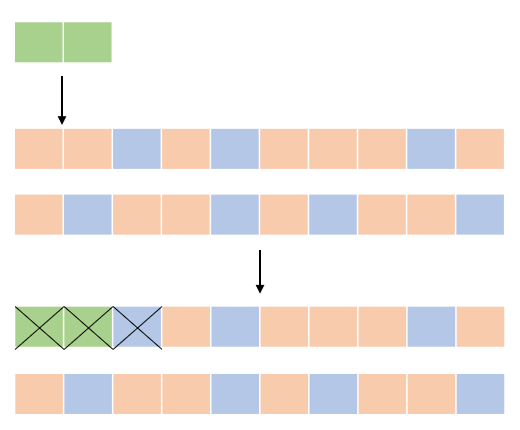
\includegraphics[width=5cm]{./Figures/seat_assign1.png}
%     \caption{Assign The Group in Row 1}
%     \end{minipage}
%     \begin{minipage}[t]{0.48\textwidth}
%     \centering
%     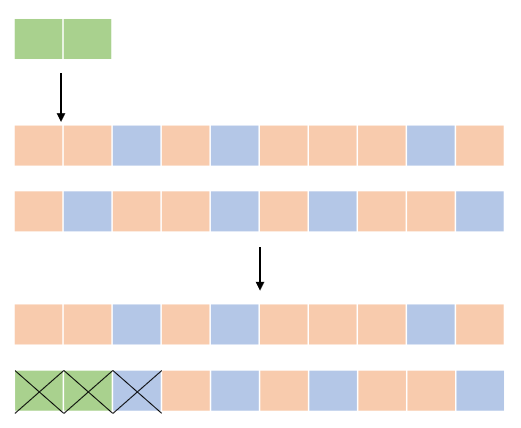
\includegraphics[width=5cm]{./Figures/seat_assign2.png}
%     \caption{Assign The Group in Row 2}
%     \end{minipage}
% \end{figure}


Our main contributions in this paper are summarized as follows. First, this study presents the first attempt to consider the arrangement of seat assignments with social distancing under dynamic arrivals. While many studies in the literature highlight the importance of social distancing in controlling the spread of the virus, they often focus too much on the model and do not provide much insight into the operational significance behind social distancing \cite{barry2021optimal, fischetti2021safe}. Recent studies have explored the effects of social distancing on health and economics, mainly in the context of aircraft \cite{salari2020social, ghorbani2020model, salari2022social}. Our study provides a new perspective to help the government adopt a mechanism for setting seat assignments to implement social distancing during pandemic.

Second, we establish a deterministic model to analyze the effects of social distancing when the demand is known. Due to the medium size of the problem, we can solve the IP model directly. We then develop the scenario-based stochastic programming by considering the stochastic demands of different group types. By using Benders decomposition methods, we can obtain the seat planning quickly. 

Third, to address the problem in the dynamic situation, we first obtain a feasible seat planning from scenario-based stochastic programming. We then make a decision for each incoming group based on our dynamic seat assignment policy, either accepting or rejecting the group. Our results demonstrate a significant improvement over the traditional control policies and provide the insights on the implementation of social distancing.

% Our results demonstrate the effectiveness of our approach in balancing social distancing requirements with revenue generation, providing valuable insights for policymakers and venue managers. Specifically, our proposed approach can help cinemas, concert venues, and other public spaces optimize seat assignments while ensuring the safety of patrons. It provides a practical tool for venues to implement social distancing measures in a flexible and efficient manner, adapting to changes in demand and maximizing revenue generation while maintaining social distancing measures.

% With this new .., we illustrate how to assign the seats by the govenment/stakeholder to balance health and economic issues. In addition, we also provide managerial guidance for the government on how to publish the related policy to make the tradeoff between economic maintenance and risk management.

The rest of this paper is structured as follows. The following section reviews relevant literature. We describe the motivating problem in Section 3. In Section 4, we establish the stochastic model,analyze its properties and obtain the seat planning. Section 5 demonstrates the dynamic seat assignment policy to assign the seats for incoming groups. Section 6 gives the numerical results and the insights of implementing social distancing. The conclusions are shown in Section 7.
\newpage


% !TEX root = sum1.tex
\section{Literature Review}\label{literature}

%The present study is closely connected to the following research areas: seat management with social distancing, multiple knapsack problem and network revenue management. The subsequent sections review the literature on each perspective and highlight significant differences between the present study and previous research.

%\subsection{Seating Management with Social Distancing}
Seating management is a practical problem that presents unique challenges in various applications, each with its own complexities, particularly when accommodating group-based seating requests. For instance, in passenger rail services, groups differ not only in size but also in their departure and arrival destinations, requiring them to be assigned consecutive seats \citep{clausen2010off, deplano2019offline}. In social gatherings such as weddings or dinner galas, individuals often prefer to sit together at the same table while maintaining distance from other groups they may dislike \citep{lewis2016creating}. In parliamentary seating assignments, members of the same party are typically grouped in clusters to facilitate intra-party communication as much as possible \citep{vangerven2022parliament}. In e-sports gaming centers, customers arrive to play games in groups and require seating arrangements that allow them to sit together \citep{kwag2022optimal}.

Incorporating social distancing into seating management has introduced an additional layer of complexity, sparking a new stream of research. Some works focus on the layout design and determine seating positions to maximize physical distance between individuals, such as students in classrooms \citep{bortolete2022support} or customers in restaurants and beach umbrella arrangements \citep{fischetti2023safe}. Other works assume the seating layout is fixed, and assign seats to individuals while adhering to social distancing guidelines. Examples include problems in air travel \citep{ghorbani2020model} and long-distance train travel \citep{haque2022optimization}. These studies underscore the growing relevance and importance of seating management in the context of social distancing.


Our work relates to seating management with social distancing for group-based requests, which has found its applications in various areas, including airplanes \citep{salari2022social}, trains \citep{haque2023social}, and theaters \citep{blom2022filling}. Due to the diversity of applications, there are different issues to handle. For example, in \cite{salari2022social}, the distance between different groups is taken into account, leading to the development of a seating assignment strategy that outperforms the simplistic airline policy of blocking all middle seats. In \citet{haque2023social}, when designing seat allocation for groups with social distancing, not only was the transmission risk inside the train considered, but also the transmission risk between different cities where the stops were located.


Our work is most closely related to \citet{blom2022filling}, as both address group-based seating problem in theaters. While in \citet{blom2022filling}, they primarily focus on scenarios with known groups - referred to as seat planning with deterministic requests in our work - we consider a broader range of demand patterns. Specifically, we also examine group-based seat planning with stochastic requests. We also consider dynamic seat assignment, assuming that groups arrive sequentially according to a stochastic process. 


%\subsection{Multiple Knapsack Problem}
When all requests are known, our problem is a special case of the multiple knapsack problem (MKP) \citep{pisinger1999exact}. It follows that some theoretical properties of MKP can be applied. However, in our problem, the knapsacks can have different capacities and there are many identical groups of the same size, thus, the aggregation form would be useful to obtain the seat plan. Furthermore, seat planning to utilize all seats is a crucial aspect of our analysis, which shows that our proposed approach will be different from those in the literature. 

% To address stochastic demand, we propose a scenario-based programming approach \cite{feng2013scenario, casey2005scenario, henrion2018problem} to determine the seat plan. Unlike existing literature, which typically considers the total supply for different demands or treats each type of supply as a protection level for corresponding demand types, we introduce a hierarchical consumption mechanism for the aggregated supply. Specifically, we adapt the constraints to reflect the hierarchical utilization of seats, where seats planned for larger groups can be repurposed for smaller groups. Additionally, the seat plan derived under demand uncertainty can serve as a reference for dynamic seat assignment, enhancing flexibility and effectiveness in real-time decision-making.

% {\bf not sure how to revise, remaining}

SADDP falls under the category of the dynamic multiple knapsack problem. When there is only one row, the problem reduces to the dynamic knapsack problem \citep{kleywegt1998dynamic}. However, there is limited research on the dynamic multiple knapsack problem, with only one mildly related study \citep{perry2009approximate}. This study models a multiperiod, single-resource capacity reservation problem by using multiple knapsacks to represent multiple time periods, which differs from our focus on the realistic multiple knapsack problem in seat assignment.

%\subsection{Network Revenue Management}
Our work is also related to the group-based \textit{network revenue management} (NRM) problem, which focuses on deciding whether to accept or reject a request \citep{gallego1997multiproduct}. The NRM problem can be fully characterized by a dynamic programming (DP) formulation. However, a significant challenge arises because the number of states grows exponentially with the problem size, rendering direct solutions computationally infeasible. To address this, various approaches have been proposed, such as deriving bid-price or booking-limit controls from static formulations or approximating the value function using simplified structures.

\citet{talluri1998analysis} was the first to propose bid-price control policies. Since then, a significant body of literature has focused on deriving refined bid prices and tighter bounds on value functions. In our work, we also consider a bid-price control policy, similar to the certainty equivalence control policy proposed by \citet{bertsimas2003revenue}, which directly uses the optimal value from a static model to approximate the initial value function. The seminal contribution to booking-limit control is from \citet{gallego1997multiproduct}, which studied a static model and introduced make-to-stock and make-to-order policies. However, these policies lack flexibility in handling stochastic demand and do not perform well for the group-based problem.


One of the key characteristics of our problem is that decisions must be made on an all-or-none basis for each group, which introduces additional complexity in handling group arrivals \citep{talluri2006theory}. Similar group-based characteristics are also observed in multi-day stays in hotel revenue management \citep{aydin2018decomposition, bitran1995application}, though the concept of a ``group'' in those contexts differs from our problem.

The introduction of group-based characteristics complicates seat management when using traditional bid-price and booking-limit control policies. Notably, in our model, the supply planned for larger groups can also be utilized by smaller groups. This flexibility stems from our approach, which focuses on group arrivals rather than individual units, distinguishing it from traditional partitioned and nested approaches \citep{curry1990optimal, van2008simulation}.

Another key characteristic of our study is the importance of seat assignment, which distinguishes it from traditional revenue management. The assign-to-seat feature introduced by \citet{zhu2023assign} further emphasizes the significance of seat assignment. This approach tackles the challenge of selling high-speed train tickets, where each request must be assigned to a specific seat for the entire journey. However, this paper focuses on individual passengers rather than groups, which sets it apart from our research.

\newpage


% !TEX root = sum1.tex
\section{Seat Planning Problem with Social Distancing}\label{problem_description}

\subsection{Concepts}
Consider $N$ knapsacks, with each knapsack $j$ containing $C_j \in \mathbb{Z}^{+}$ capacities, for $j \in \mathcal{N} \coloneqq \{1,2, \ldots, N\}$. There are $M$ distinct item types, where each item type $i$, $i \in \mathcal{M} \coloneqq \{1, 2, \ldots, M\}$, requiring $w_i \in \mathbb{Z}^{+}$ consecutive size in one capacity. The profit of each item type $i$ is $r_{i} \in \mathbb{Z}^{+}$. The request of each item type is represented by a demand vector $\mathbf{d} = (d_1, d_2, \ldots, d_M)^{\intercal}$, where $d_i$ is the number of groups of type $i$.

We now formulate the multi-class multiple knapsack problem (MMKP) as an integer programming, where $x_{ij}$ represents the number of items of type $i$ placed in knapsack $j$.

\begin{align}
(\text{MMKP}) \quad \max \quad & \sum_{i=1}^{M}  \sum_{j= 1}^{N} r_{i} x_{ij} \label{e0} \\
\text {s.t.} \quad & \sum_{j= 1}^{N} x_{ij} \leq d_{i}, \quad i \in \mathcal{M}, \label{deter_upper}\\ 
& \sum_{i=1}^{M} w_{i} x_{ij} \leq C_j, j \in \mathcal{N}, \label{capa_con} \\
& x_{ij} \in \mathbb{N}, \quad i \in \mathcal{M}, j \in \mathcal{N}. \notag 
\end{align}


The objective function (\ref{e0}) is to maximize the number of individuals accommodated. Constraint \eqref{deter_upper} ensures the total number of accommodated groups does not exceed the number of requests for each group type. Constraint \eqref{capa_con} stipulates that the number of seats allocated in each row does not exceed the size of the row.


Suppose that the profit-weight ratio is increasing monotone. The increasing nature of the ratio $\frac{r_i}{w_i}$ with respect to type $i$ leads to preferential inclusion of larger items in the optimal fractional assignment. This intuitive property is illustrated in Proposition \ref{sol_relax_deter}. 

% By examining the monotonic ratio of $\frac{i}{n_i}$, we can establish the upper bound of supply corresponding to the optimal solution of the LP relaxation of SPDR problem.

\begin{prop}\label{sol_relax_deter}
For the LP relaxation of the \textup{MMKP} problem, there exists an index $\tilde{i}$ such that the optimal solutions satisfy the following conditions: $x_{ij}^{*} = 0$ for all $j$, $i = 1,\ldots, \tilde{i}-1$; $\sum_{j=1}^{N} x_{ij}^{*} = d_{i}$ for $i = \tilde{i}+1,\ldots, M$; $\sum_{j=1}^{N} x_{ij}^{*} = \frac{L - \sum_{i = \tilde{i}+1}^{M} {d_i w_i}}{w_{\tilde{i}}}$ for $i = \tilde{i}$.
\end{prop}

% !TEX root = ./sum1.tex
% \section{Stochastic Demands Situation}

\section{Scenario-based Stochastic Programming}
This section focuses on seat planning in scenarios with varying demand. We begin by introducing a scenario-based stochastic programming formulation. However, due to its time-consuming nature, we transform it into a two-stage problem and implement benders decomposition to obtain the optimal linear solution. Using this solution, we generate a feasible seat planning.

\subsection{Formulation}
Now suppose the demand of groups is stochastic, the stochastic information can be obtained from scenarios through historical data. Use $\omega$ to index the different scenarios, each scenario $\omega \in \Omega$. A particular realization of the demand vector can be represented as $\mathbf{d}_\omega = (d_{1\omega},d_{2\omega},\ldots,d_{M,\omega})^{\intercal}$. Let $p_{\omega}$ denote the probability of any scenario $\omega$, which we assume to be positive. To maximize the expected value of people over all the scenarios, we propose a scenario-based stochastic programming.

Consider the decision makers who give the seat planning based on the scenarios then assign the groups to seats according to the realized true demand. 

The seat planning can be denoted by decision variables $\mathbf{x}\in \mathbb{Z}_{+}^{M \times N}$. Let $x_{i,j}$ stand for the number of group type $i$ in row $j$. The supply for group type $i$ can be represented by $\sum_{j=1}^N x_{ij}$.
Regarding the nature of the obtained information, we assume that there are $S = |\Omega|$ possible scenarios. There is a scenario-dependent decision variable, $\mathbf{y}$, to be chosen. It includes two vectors of decisions, $\mathbf{y}^{+} \in \mathbb{Z}_{+}^{M \times S}$ and $\mathbf{y}^{-} \in \mathbb{Z}_{+}^{M \times S}$. Each component of $\mathbf{y}^{+}$, $y_{i}^{\omega(+)}$, represents the number of surplus seats for group type $i$. Similarly, $y_{i}^{\omega(-)}$ represents the number of inadequate seats for group type $i$.
Considering that the group can take the seats planned for the larger group type, we assume that the surplus seats for group type $i$ can be occupied by smaller group type $j<i$ in the descending order of the group size. That is, for any $\omega$, $i \leq M-1$, $y_{i \omega}^{+}=\left(\sum_{j=1}^N x_{ij}- d_{i \omega} + y_{i+1, \omega}^{+}\right)^{+}$ and $y_{i \omega}^{-}=\left(d_{i \omega}- \sum_{j=1}^N x_{ij} - y_{i+1, \omega}^{+} \right)^{+}$, where $(x)^{+}$ equals $x$ if $x>0$, $0$ otherwise. Specially, for the largest group type $M$, we have $y_{M \omega}^{+} = (\sum_{j=1}^N x_{ij} - d_{i \omega})^{+}$, $y_{M \omega}^{-} = (d_{i \omega}- \sum_{j=1}^N x_{ij})^{+}$.

% These variables are scenario-independent and 

% Because the demand is unknown when the seat assignment is planned, there is no way to expect that the supply in the first stage can meet the demand exactly. Fortunately, we can find some remedies in practice, for example, seats of 5 can be assigned to a group of 4 with one empty seat as social distancing. However, the decision maker will confront seats shortage or excess without these measures. Therefore, to deal with possible demands, the wait-and-see measures (called recourses) should be considered in planning seat assignment.

% If no group of 1 comes in the future, this wait-and-see measure may leave two empty seats. 

% and that the true demand is only revealed after $\mathbf{x}$ is chosen.

% which is positive when the supply is larger than the actual demand, zero otherwise.
% which is positive when the supply is less than the actual demand and zero otherwise.

% which include the number of holding groups, $y_{i \omega}^{+}$, positive when the supply overestimates the actual demand and the number of short groups, $y_{i \omega}^{-}$, positive when the supply understimates the actual demand for group type $i$ in scenario $\omega$.

% The assignment will be determined before the realization of the random demand, here-and-now policy.

Then we have the deterministic equivalent form(DEF) of the scenario-based stochastic programming:
    \begin{align}
    (DEF) \quad \max \quad & E_{\omega}\left[\sum_{i=1}^{M-1} (n_i-\delta) (\sum_{j= 1}^{N} x_{ij} + y_{i+1,\omega}^{+} - y_{i \omega}^{+}) + (n_{M}-\delta) (\sum_{j= 1}^{N} x_{Mj} - y_{M \omega}^{+})\right] \\
    \text {s.t.} \quad & \sum_{j= 1}^{N} x_{ij}-y_{i \omega}^{+}+
    y_{i+1, \omega}^{+} + y_{i \omega}^{-}=d_{i \omega}, \quad i = 1,\ldots, M-1, \omega \in \Omega \label{DEF_constr1} \\
    & \sum_{j= 1}^{N} x_{ij} -y_{i \omega}^{+}+y_{i \omega}^{-}=d_{i \omega}, \quad i = M, \omega \in \Omega \label{DEF_constr2}\\
    & \sum_{i=1}^{M} n_{i} x_{ij} \leq L_j, j \in \mathcal{N}  \label{DEF_constr3} \\
    & y_{i \omega}^{+}, y_{i \omega}^{-} \in \mathbb{Z}_{+}, \quad i \in \mathcal{M}, \omega \in \Omega \\
    & x_{ij} \in \mathbb{Z}_{+}, \quad i \in \mathcal{M}, j \in \mathcal{N}.
    \end{align}

The objective function contains two parts, the number of the largest group type that can be accommodated is $\sum_{j= 1}^{N} x_{Mj} - y_{M \omega}^{+}$. The number of group type $i$ that can be accommodated is $\sum_{j= 1}^{N} x_{ij} + y_{i+1,\omega}^{+} - y_{i \omega}^{+}$. $E_{\omega}$ is the expectation with respect to the scenario set.

By reformulating the objective function, we have

\begin{align*}
  & E_{\omega}\left[\sum_{i=1}^{M-1} (n_i-\delta) (\sum_{j= 1}^{N} x_{ij} + y_{i+1,\omega}^{+} - y_{i \omega}^{+}) + (n_M-\delta) (\sum_{j= 1}^{N} x_{Mj} - y_{M \omega}^{+})\right] \\
  =& \sum_{j =1}^{N} \sum_{i=1}^M (n_i- \delta) x_{ij} - \sum_{\omega =1}^{S} p_{\omega} \left(\sum_{i=1}^{M}(n_i- \delta)y_{i \omega}^{+} - \sum_{i=1}^{M-1}(n_i-\delta)y_{i+1, \omega}^{+}\right) \\
  =& \sum_{j =1}^{N} \sum_{i=1}^M i \cdot x_{ij} - \sum_{\omega =1}^{S} p_{\omega} \sum_{i = 1}^{M} y_{i \omega}^{+}
\end{align*}

% Plug in $s_i = i+1$, the objective function is $\sum_{j =1}^{N} \sum_{i=1}^m i x_{ij} - \sum_{\omega =1}^{S} p_{\omega} \sum_{i=1}^{m} y_{i \omega}^{+}$.

The last equality holds because of $n_i- \delta = i, i \in \mathcal{M}$. 

\begin{remark}
For any $i, \omega$, at most one of $y_{i \omega}^{+}$ and $y_{i \omega}^{-}$ can be positive. 
Suppose there exist $i_0$ and $\omega_0$ such that $y_{i_0 \omega_0}^{+}$ and $y_{i_0 \omega_0}^{-}$ are positive. Substracting $\min\{y_{i_0, \omega_0}^{+}, y_{i_0, \omega_0}^{-}\}$ from these two values will still satisfy constraints \eqref{DEF_constr1} and \eqref{DEF_constr2} but increase the objective value when $p_{\omega_0}$ is positive. Thus, at most one of $y_{i \omega}^{+}$ and $y_{i \omega}^{-}$ can be positive. 
\end{remark}

Let $\mathbf{n} = (n_1, \ldots, n_M)$, $\mathbf{L} = (L_1, \ldots, L_N)$ where $s_i$ is the size of seats taken by group type $i$ and $L_j$ is the length of row $j$ as we defined above. Then the constraint \eqref{DEF_constr3} can be expressed as $\mathbf{n} \mathbf{x} \leq \mathbf{L}$.

The linear constraints associated with scenarios, i.e., constraints \eqref{DEF_constr1} and \eqref{DEF_constr2}, can be written in a matrix form as
\[\mathbf{x} \mathbf{1} + \mathbf{V} \mathbf{y}_\omega = \mathbf{d}_\omega, \omega\in \Omega,\]

where $\mathbf{1}$ is a column vector of size $N$ with all 1s, $\mathbf{V} = [\mathbf{W}, ~\mathbf{I}]$.

$$
\mathbf{W}=\left[\begin{array}{ccccc}
-1 & 1 & \ldots & & 0 \\
& \ddots & \ddots & & \vdots \\
& & & & 1 \\
0 & & & & -1
\end{array}\right]_{M \times M}
$$

and $\mathbf{I}$ is the identity matrix. For each scenario $\omega \in \Omega$,
$$
\mathbf{y}_{\omega}=\left[\begin{array}{l}
\mathbf{y}_{\omega}^{+} \\
\mathbf{y}_{\omega}^{-}
\end{array}\right], \mathbf{y}_{\omega}^{+}=\left[\begin{array}{lllll}y_{1 \omega}^{+} & y_{2 \omega}^{+} & \cdots & y_{M \omega}^{+}\end{array}\right]^{\intercal}, \mathbf{y}_{\omega}^{-}=\left[\begin{array}{llll}y_{1 \omega}^{-} & y_{2 \omega}^{-} & \cdots & y_{M \omega}^{-}\end{array}\right]^{\intercal}.
$$

As we can find, this deterministic equivalent form is a large-scale problem even if the number of possible scenarios $\Omega$ is moderate. However, the structured constraints allow us to simplify the problem by applying Benders decomposition approach. Before using this approach, let us write this problem in the form of the two-stage stochastic programming.

Let $\mathbf{c}^{\intercal}\mathbf{x} = \sum_{j =1}^{N} \sum_{i=1}^M i \cdot x_{ij}$, $\mathbf{f}^{\intercal}\mathbf{y}_{\omega} = -\sum_{i=1}^{M} y_{i \omega}^{+}$. Then the DEF formulation can be expressed as below,

\begin{equation}\label{BD_master}
  \begin{aligned}
\max \quad & \mathbf{c}^{\intercal} \mathbf{x}+ z(\mathbf{x}) \\
\text {s.t.} \quad & \mathbf{n} \mathbf{x} \leq \mathbf{L} \\
& \mathbf{x} \in \mathbb{Z}_{+}^{M \times N},
\end{aligned}
\end{equation}

where $z(\mathbf{x})$ is the recourse function defined as 

$$z(\mathbf{x}) := E(z_{\omega}(\mathbf{x})) = \sum_{\omega \in \Omega} p_{\omega} z_{\omega}(\mathbf{x}),$$ and for each scenario $\omega \in \Omega$, 

\begin{equation}\label{BD_sub}
  \begin{aligned}
    z_{\omega}(\mathbf{x}) := \max \quad & \mathbf{f}^{\intercal} \mathbf{y}_{\omega} \\
    \text {s.t.} \quad & \mathbf{x} \mathbf{1} + \mathbf{V} \mathbf{y}_{\omega} = \mathbf{d}_{\omega} \\
     & \mathbf{y}_{\omega} \geq 0.
  \end{aligned}
  \end{equation}

% The objective function of problem \eqref{sto_form} can be expressed as $c{'}\mathbf{x} + \sum_{\omega} p_{\omega}f{'}y_{\omega}$. 
Problem \eqref{BD_sub} stands for the second-stage problem and $z_{\omega}(\mathbf{x})$ is the optimal value of problem \eqref{BD_sub}, together with the convention $z_{\omega}(\mathbf{x}) = \infty$ if the problem is infeasible.

Solving the above problem directly can be challenging, so we first obtain the optimal solution to the relaxation of problem \eqref{BD_master}. From this solution, we generate a seat planning.

\subsection{Solve the Scenario-based Two-stage Problem}\label{solve_by_benders}
At first, we generate a closed-form solution to the second-stage problem in section \ref{second_stage}. Then we obtain the solution to the linear relaxation of problem \eqref{BD_master} by the delayed constraint generation. Finally, we obtain a feasible seat planning from the linear solution.

\subsubsection{Solve the Second Stage Problem}\label{second_stage}

Consider a $\mathbf{x}$ such that $\mathbf{n x} \leq \mathbf{L}$ and $\mathbf{x} \geq 0$ and suppose that this represents the seat planning. Once $\mathbf{x}$ is fixed, the optimal decisions $\mathbf{y}_{\omega}$ can be determined by solving problem \eqref{BD_sub} for each $\omega$.

% To solve this problem, we should only consider that $\mathbf{x}$ for which $z_{\omega}(\mathbf{x})$ are all finite. 
Notice that the feasible region of the dual of problem \eqref{BD_sub} does not depend on $\mathbf{x}$. Let $\bm{\alpha}$ be the vector of dual variable. For each $\omega$, we can form its dual problem, which is 

\begin{equation}\label{BD_sub_dual}
  \begin{aligned}
    \min \quad & \bm{\alpha}^{\intercal} (\mathbf{d}_{\omega}- \mathbf{x} \mathbf{1}) \\
    \text {s.t.} \quad & \bm{\alpha}^{\intercal} \mathbf{V} \geq \mathbf{f}^{\intercal}
  \end{aligned}
  \end{equation}

Let $\mathbb{P} = \{\bm{\alpha} \in \mathbb{R}^{M}|\bm{\alpha}^{\intercal} \mathbf{V} \geq \mathbf{f}^{\intercal}\}$. 
We assume that $\mathbb{P}$ is nonempty and has at least one extreme point. Then, either the dual problem \eqref{BD_sub_dual} has an optimal solution and $z_{\omega}(\mathbf{x})$ is finite, or the primal problem \eqref{BD_sub} is infeasible and $z_{\omega}(\mathbf{x}) = \infty$.  

Let $\mathcal{O}$ be the set of all extreme points of $\mathbb{P}$ and $\mathcal{F}$ be the set of all extreme rays of $\mathbb{P}$. Then $z_{\omega} > -\infty$ if and only if $\bm{\alpha}^{\intercal}(\mathbf{d}_{\omega}- \mathbf{x} \mathbf{1}) \geq 0, \bm{\alpha} \in \mathcal{F}$, which stands for the feasibility cut.

\begin{lem}\label{feasible_region}
  The feasible region of problem \eqref{BD_sub_dual}, $\mathbb{P}$, is bounded. In addition, all the extreme points of $\mathbb{P}$ are integral.
\end{lem}

\begin{pf}[Proof of lemma \ref{feasible_region}]
Notice that $\mathbf{f}^{\intercal} = [-\mathbf{1},~\mathbf{0}], V =[W,~I]$, $W$ is a totally unimodular matrix. Then, we have $\bm{\alpha}^{\intercal}W \geq -\mathbf{1}, \bm{\alpha}^{\intercal} I \geq \mathbf{0}$. Thus, the feasible region is bounded. 
Furthermore, let $\alpha_0 = 0$, then we have $0 \leq \alpha_i \leq \alpha_{i-1} +1$, $i \in \mathcal{M}$, so the extreme points are all integral.
\qed
\end{pf}

Because the feasible region is bounded, then feasibility cuts are not needed. Let $z_{\omega}$ be the lower bound of $z_{\omega}(x)$ such that $\bm{\alpha}^{\intercal}(\mathbf{d}_{\omega}- \mathbf{x} \mathbf{1}) \geq z_{\omega}, \bm{\alpha} \in \mathcal{O}$, which is the optimality cut.

\begin{corollary}
  Only the optimality cuts, $\alpha^{\intercal}(\mathbf{d}_{\omega}- \mathbf{x} \mathbf{1}) \geq z_{\omega}$, will be included in the decomposition approach.
\end{corollary}

\begin{corollary}
The optimal value of the problem \eqref{BD_sub}, $z_{\omega}(x)$, is finite and will be attained at extreme points of the set $P$. Thus, we have $z_{\omega}(x) = \min_{\bm{\alpha} \in \mathcal{O}} \bm{\alpha}^{\intercal}(\mathbf{d}_{\omega}- \mathbf{x} \mathbf{1})$. 
\end{corollary}


When we are given $\mathbf{x}^{*}$, the demand that can be satisfied by the assignment is $\mathbf{x}^{*} \mathbf{1} = \mathbf{d}_0 = (d_{1,0},\ldots,d_{M,0})^{\intercal}$.
Then plug them in the subproblem \eqref{BD_sub}, we can obtain the value of $y_{i \omega}$ recursively:
\begin{equation}\label{y_recursively}
\begin{aligned}
  & y_{M \omega}^{-}=\left(d_{M \omega}-d_{M 0}\right)^{+} \\
  & y_{M \omega}^{+}=\left(d_{M 0}-d_{M \omega}\right)^{+} \\
  & y_{i \omega}^{-}=\left(d_{i \omega}-d_{i 0} - y_{i+1, \omega}^{+} \right)^{+}, i =1,\ldots, M-1 \\
  & y_{i \omega}^{+}=\left(d_{i 0}- d_{i \omega} + y_{i+1, \omega}^{+}\right)^{+}, i =1,\ldots, M-1
\end{aligned}
\end{equation}

The optimal value for scenario $\omega$ can be obtained by $\mathbf{f}^{\intercal} y_{\omega}$, then we need to find the dual optimal solution.


\begin{thm}\label{optimal_sol_sub_dual}
  The optimal solutions to problem \eqref{BD_sub_dual} are given by 
\begin{equation}\label{BD_sub_simplified}
  \begin{aligned}
    & \alpha_{i} = 0, i \in \mathcal{M} \quad \text{if}~  y_{i \omega}^{-} > 0,  y_{i \omega}^{+} = 0   \\
    & \alpha_{i} = \alpha_{i-1}+1, i \in \mathcal{M} \quad \text{if}~ y_{i \omega}^{+} > 0,  y_{i \omega}^{-} = 0 \\
    & \alpha_{i} = 0, i =1,\ldots, M-1 \quad \text{if}~ y_{i \omega}^{-} = y_{i \omega}^{+} = 0, y_{i+1, \omega}^{+}> 0 \\
    & 0 \leq \alpha_{i} \leq \alpha_{i-1}+1, i =1,\ldots, M-1 \quad \text{if}~ y_{i \omega}^{-} = y_{i \omega}^{+} = 0, y_{i+1, \omega}^{+}= 0 \\
    & 0 \leq \alpha_{i} \leq \alpha_{i-1}+1, i = M \quad \text{if}~ y_{i \omega}^{-} = y_{i \omega}^{+} = 0
  \end{aligned}
\end{equation}
\end{thm}

\begin{pf}[Proof of Theorem \ref{optimal_sol_sub_dual}]
According to the complementary slackness property, we can obtain the following equations
\begin{align*}
  & \alpha_{i} (d_{i0} - d_{i \omega} - y_{i \omega}^{+} + y_{i+1, \omega}^{+} + y_{i \omega}^{-}) = 0, i =1,\ldots, M-1 \\
  & \alpha_{i} (d_{i0} - d_{i \omega} - y_{i \omega}^{+}+ y_{i \omega}^{-}) = 0, i = M \\
  & y_{i \omega}^{+}(\alpha_{i} - \alpha_{i-1}-1) = 0, i =1,\ldots, M \\
  & y_{i \omega}^{-} \alpha_{i} = 0, i =1,\ldots, M.
\end{align*}

When $y_{i \omega}^{-} >0$, we have $\alpha_{i} =0$; when $y_{i \omega}^{+} >0$, we have $\alpha_{i} = \alpha_{i-1} +1$.
Let $\Delta d = d_{\omega} - d_0$, then the elements of $\Delta d$ will be a negative integer, positive integer and zero.
When $y_{i \omega}^{+} = y_{i \omega}^{-} = 0$, if $i = M$, $\Delta d_{M} =0$, the value of objective function associated with $\alpha_{M}$ is always $0$, thus we have $0 \leq \alpha_{M} \leq \alpha_{M-1}+1$; if $i < M$, we have $y_{i+1, \omega}^{+} = \Delta d_{i} \geq 0$. If $y_{i+1, \omega}^{+} > 0$, the objective function associated with $\alpha_i$ is $\alpha_{i} \Delta d_{i} = \alpha_{i} y_{i+1, \omega}^{+}$, thus to minimize the objective value, we have $\alpha_i =0$; if $y_{i+1, \omega}^{+} = 0$, we have $0 \leq \alpha_{i} \leq \alpha_{i-1} +1$.
\qed
\end{pf}

% \begin{remark}
% During the calculation, we choose the optimal solution $\alpha_{i} = \alpha_{i-1} +1$ when $0 \leq \alpha_{i} \leq \alpha_{i-1} +1$.
% \end{remark}

We can use the forward method, calculating from $\alpha_{1 \omega}$ to $\alpha_{M \omega}$, to obtain the value of $\alpha_{\omega}$ instead of solving the original large-scale linear programming.

\subsubsection{Delayed Constraint Generation}\label{bender_stage}
Benders decomposition works with only a subset of those exponentially many constraints and adds more constraints iteratively until the optimal solution of Benders Master Problem(BMP) is attained. This procedure is known as delayed constraint generation.

% Restricted Benders master problem:
Use the characterization of $z_{\omega}(x)$ in the problem \eqref{BD_master} and take into account the optimality cuts, we can conclude the BMP will have the form:

\begin{equation}\label{BD_master2}
  \begin{aligned}
    \max \quad & \mathbf{c}^{\intercal} \mathbf{x} + \sum_{\omega \in \Omega} p_{\omega} z_{\omega} \\
    \text {s.t.} \quad & \mathbf{n} \mathbf{x} \leq \mathbf{L} \\
    & \bm{\alpha}^{\intercal}(\mathbf{d}_{\omega}- \mathbf{x} \mathbf{1}) \geq z_{\omega}, \bm{\alpha} \in \mathcal{O}, \forall \omega \\
     & \mathbf{x} \geq 0, z_{\omega} ~\text{is free}
  \end{aligned}
\end{equation}

When substituting $\mathcal{O}$ with its subset, $\mathcal{O}^{t}$, the problem \eqref{BD_master2} becomes the Restricted Benders Master Problem(RBMP). 

To determine the initial $\mathcal{O}^{t}$, we have the following lemma.

\begin{lem}\label{one_ep_feasible}
RBMP is always bounded with at least any one optimality cut for each scenario.
\end{lem}

\begin{pf}[Proof of lemma \ref{one_ep_feasible}]
  Suppose we have one extreme point $\bm{\alpha}_{\omega}^{0}$ for each scenario. Then we have the following problem.
  \begin{equation}\label{lemma_eq}
    \begin{aligned}
      \max \quad & \mathbf{c}^{\intercal} \mathbf{x} + \sum_{\omega \in \Omega} p_{\omega} z_{\omega} \\
      \text {s.t.} \quad & \mathbf{n} \mathbf{x} \leq \mathbf{L} \\
      & (\bm{\alpha}_{\omega}^{0})^{\intercal}\mathbf{d}_{\omega} \geq (\bm{\alpha}_{\omega}^{0})^{\intercal} \mathbf{x} \mathbf{1} + z_{\omega}, \forall \omega \\
       & \mathbf{x} \geq 0
    \end{aligned}
  \end{equation}
  Problem \eqref{lemma_eq} reaches its maximum when $(\bm{\alpha}_{\omega}^{0})^{\intercal}\mathbf{d}_{\omega} = (\bm{\alpha}_{\omega}^{0})^{\intercal} \mathbf{x} \mathbf{1} + z_{\omega}, \forall \omega$. Substitute $z_{\omega}$ with these equations, we have 
  \begin{equation}\label{lemma_eq2}
    \begin{aligned}
      \max \quad & \mathbf{c}^{\intercal} \mathbf{x} - \sum_{\omega}p_{\omega}(\bm{\alpha}_{\omega}^{0})^{\intercal} \mathbf{x} \mathbf{1} + \sum_{\omega} p_{\omega} (\bm{\alpha}_{\omega}^{0})^{\intercal} \mathbf{d}_{\omega} \\
      \text {s.t.} \quad & \mathbf{n} \mathbf{x} \leq \mathbf{L} \\
      & \mathbf{x} \geq 0
    \end{aligned}
  \end{equation}
  Notice that $\mathbf{x}$ is bounded by $\mathbf{L}$, then the problem \eqref{lemma_eq} is bounded. Adding more optimality cuts will not make the optimal value larger. Thus, RBMP is bounded. 
  \qed
\end{pf}

Given the initial $\mathcal{O}^{t}$, we can have the solution $\mathbf{x}_{0}$ and $\mathbf{z}^{0} =(z^{0}_1,\ldots, z^{0}_S)$. Then $c^{\intercal} \mathbf{x}_0 + \sum_{\omega \in \Omega} p_{\omega} z_{\omega}^{0}$ is an upper bound of problem \eqref{BD_master2}. 


When $\mathbf{x}_0$ is given, the optimal solution, $\bm{\alpha}_{\omega}^{1}$, to problem \eqref{BD_sub_dual} can be obtained according to Theorem \ref{optimal_sol_sub_dual}. $z_{\omega}^{(0)} = \bm{\alpha}_{\omega}^{1}(d_{\omega} - \mathbf{x}_0 \mathbf{1})$ and $(\mathbf{x}_0, \mathbf{z}^{(0)})$ is a feasible solution to problem \eqref{BD_master2} because it satisfies all the constraints. Thus, $\mathbf{c}^{\intercal} \mathbf{x}_0 + \sum_{\omega \in \Omega} p_{\omega} z_{\omega}^{(0)}$ is a lower bound of problem \eqref{BD_master2}.

If for every scenario $\omega$, the optimal value of the corresponding problem \eqref{BD_sub_dual} is larger than or equal to $z_{\omega}^{0}$, all contraints are satisfied, we have an optimal solution, $(\mathbf{x}_{0}, \mathbf{z}_{\omega}^{0})$, to the BMP. Otherwise, add one new constraint, $(\bm{\alpha}_{\omega}^{1})^{\intercal}(\mathbf{d}_{\omega}- \mathbf{x} \mathbf{1}) \geq z_{\omega}$, to RBMP.

% $z_{\omega}^{(0)} = \alpha_{\omega}^{*}(d_{\omega} - \mathbf{x}_0 \mathbf{1})$ will give a minimal upper bound of $z_{\omega}$, thus all the left constraints associated with other extreme points are redundant.when the extreme points are $\alpha_{\omega}$.

% The problem \eqref{lemma_eq} associated with $\alpha_{\omega}$ will give an optimal solution $(x_1, z_{\omega}^{1})$. (Upper bound)


The steps of the algorithm are described as below,

\begin{algorithm}[H]\label{cut_algo}
  \caption{The benders decomposition algorithm}
    \begin{description}
    \item[Step 1.] Solve LP \eqref{lemma_eq} with all $\alpha_{\omega}^0 = \mathbf{0}$ for each scenario. Then, obtain the solution $(\mathbf{x}_0, \mathbf{z}^{0})$.
    \item[Step 2.] Set the upper bound $UB = c^{\intercal} \mathbf{x}_0 + \sum_{\omega \in \Omega} p_{\omega} z_{\omega}^{0}$.
    \item[Step 3.] For $x_0$, we can obtain $\alpha_{\omega}^{1}$ and $z_{\omega}^{(0)}$ for each scenario, set the lower bound $LB = c^{\intercal} x_0 + \sum_{\omega \in \Omega} p_{\omega} z_{\omega}^{(0)}$.
    \item[Step 4.] For each $\omega$, if $(\alpha_{\omega}^{1})^{\intercal}(\mathbf{d}_{\omega}- \mathbf{x}_0 \mathbf{1}) < z_{\omega}^{0}$, add one new constraint, $(\alpha_{\omega}^{1})^{\intercal}(\mathbf{d}_{\omega}- \mathbf{x} \mathbf{1}) \geq z_{\omega}$, to RBMP.
    \item[Step 5.] Solve the updated RBMP, obtain a new solution $(x_1, z^{1})$ and update UB.
    \item[Step 6.] Repeat step 3 until $UB - LB < \epsilon$.(In our case, UB converges.)
   \end{description}
  \end{algorithm}

\begin{remark}
From the Lemma \ref{one_ep_feasible}, we can set $\bm{\alpha}_{\omega}^0 = \mathbf{0}$ initially in {\bf Step 1}.
\end{remark}

\begin{remark}
Notice that only contraints are added in each iteration, thus $LB$ and $UB$ are both monotone. Then we can use $UB - LB < \epsilon$ to terminate the algorithm in {\bf Step 6}.
\end{remark}

After the algorithm terminates, we obtain the optimal $\mathbf{x}^{*}$. The demand that can be satisfied by the arrangement is $\mathbf{x}^{*} \mathbf{1} = \mathbf{d}_0 = (d_{1,0},\ldots,d_{M,0})$.
Then we can obtain the value of $\mathbf{y}_{\omega}$ from equation \eqref{y_recursively}.

% We show the results of Benders and IP in the section \ref{Bender_IP}.

\subsection{Obtain the Feasible Seat Planning}\label{seat_assignment}
The decomposition method only gives a fractional solution and the stochastic model does not provide an appropriate seat planning when the number of people in scenario demands is way smaller than the number of the seats. Thus, we change the linear solution from the decomposition method to obtain a feasible seat planning. Before that, we will discuss the deterministic model that can help to achieve the goal.

% The objective is to obtain the maximal number of people placed according to the demand scenarios. It will not provide an appropriate seat assignment when the number of people associated with scenario demands is way less than the number of available seats because there are multiple optimal solutions and the solution given by solver probably does not utilize all the empty seats.

When $|\Omega| =1$ in DEF formulation, the stochastic programming will be 

\begin{equation}\label{one_form}
  \begin{aligned}
  \max \quad & \sum_{i=1}^{M}  \sum_{j= 1}^{N} (n_i-\delta) x_{ij} - \sum_{i=1}^{M} y_{i}^{+}  \\
  \text {s.t.} \quad & \sum_{j= 1}^{N} x_{ij} - y_{i}^{+}+ y_{i+1}^{+} + y_{i}^{-} = d_{i}, \quad i = 1, \ldots, M-1, \\
  & \sum_{j= 1}^{N} x_{ij} -y_{i}^{+} + y_{i}^{-} = d_{i}, \quad i = M, \\
  & \sum_{i=1}^{M} n_{i} x_{ij} \leq L_j, j \in \mathcal{N}\\
  & y_{i}^{+}, y_{i}^{-} \in \mathbb{Z}_{+}, \quad i \in \mathcal{M} \\
  & x_{ij} \in \mathbb{Z}_{+}, \quad i \in \mathcal{M}, j \in \mathcal{N}.
  \end{aligned}
\end{equation}

To maximize the objective function, we can take $y_i^{+} = 0$. Notice that $y_{i}^{-} \geq 0$, thus the constraints $\sum_{j= 1}^{N} x_{ij} + y_{i}^{-} = d_{i}, i \in \mathcal{M}$ can be rewritten as $\sum_{j= 1}^{N} x_{ij} \leq d_{i}, i \in \mathcal{M}$, then we have

\begin{equation}\label{deter_upper}
  \begin{aligned}
  \max \quad & \sum_{i=1}^{M}  \sum_{j= 1}^{N} (n_i- \delta) x_{ij} \\
  \text {s.t.} \quad & \sum_{j= 1}^{N} x_{ij} \leq d_{i}, \quad i \in \mathcal{M}, \\
  & \sum_{i=1}^{M} n_{i} x_{ij} \leq L_j, j \in \mathcal{N} \\
  & x_{ij} \in \mathbb{Z}_{+}, \quad i \in \mathcal{M}, j \in \mathcal{N}.
  \end{aligned}
\end{equation}

Problem \eqref{deter_upper} represents the deterministic model. Demand, $d_i, i \in \mathcal{M}$ is known in advance, our goal is to accommodate as many as people possible in the fixed rows.

\begin{lem}\label{sol_relax_deter}
For the linear relaxation of problem \eqref{deter_upper}, there exists $h$ such that the optimal solutions $x_{ij}^{*} = 0$ when $i < h$; $\sum_{j} x_{ij}^{*} = d_{i}$, when $i > h$; $\sum_{j} x_{ij}^{*} = (L - \sum_{i = h+1}^{M} {d_i n_i})/ n_h$, when $i = h$.
\end{lem}

Let $\sum_{j=1}^{N} x_{ij}$ represent the supply for group type $i$. We define $\mathbf{X} = (\sum_{j=1}^{N} x_{1j},\ldots, \sum_{j=1}^{N} x_{Mj})$ as the aggregate solution to the linear relaxation of problem \eqref{deter_upper}. Furthermore, let $e_{i}$ denote the unit size of the $i$-th element of $\mathbf{X}$.

In the aggregate optimal solution, denoted as $x e_{h} + \sum_{i=h+1} ^{M} d_{i} e_{i}$, the following components are present: $x e_{h}$: This term represents the allocation of resources for group type $h$. The value of $x$ is calculated as $(L- \sum_{i = h+1}^{M} {d_i n_i})/ n_h$, indicating the remaining capacity after satisfying the demands of indices greater than $h$, divided by the unit size $n_h$. $\sum_{i=h+1} ^{M} d_{i} e_{i}$: This term accounts for the allocation of resources for group types $h+1$ to $M$. It represents the total demand for these group types, where $d_i$ denotes the demand of group type $i$, and $e_{i}$ represents the unit size of the corresponding element in $\mathbf{X}$. Together, the aggregate optimal solution combines the allocation of resources for group type $h$ with the aggregated demands for group types $h+1$ to $M$ to achieve an optimal solution to the linear relaxation of the problem.

% Suppose that each row has the same length. Then the optimal integrated solution 
% $(0,\ldots, x,d_{h+1}, \ldots, d_{m})$ has the same objective value with an integer solution. Deciding if these items can fit into a specified number of rows is the decision problem of the bin-packing problem. If the items associated with the integer solution can be put in the given number of rows, this solution is optimal; otherwise, it is not optimal. Since the bin-packing problem is NP-hard, problem \eqref{deter_upper} is also NP-hard.

% its objective is to obtain the maximal number of people served, not the optimal seat assignment. It will not provide an appropriate solution when the number of arriving people in the scenarios is way less than the number of total seats because it does not utilize all the empty seats.

Let the optimal solution to the relaxation of DEF be $x^{*}_{ij}$. Aggregate $\mathbf{x}^{*}$ to the number of each group type, ${s}_{i}^{0} =\sum_{j} x^{*}_{ij}, i \in \mathbf{M}$. Replace the vector $\mathbf{d}$ with $\mathbf{s}^{0}$, we have the following problem, 

\begin{equation}\label{deter_upper1}
  \{\max \sum_{j=1}^{N} \sum_{i=1}^{M}(n_i -\delta) x_{ij}: \sum_{i = 1}^{M} n_i x_{ij} \leq L_{j}, j \in \mathcal{N}; \sum_{j =1}^{N} x_{ij} \leq s_{i}^{0}, i \in \mathcal{M}; x_{ij} \in Z^{+} \}
\end{equation}

then solve the resulting problem \eqref{deter_upper1} to obtain the optimal solution, $\mathbf{x}^{1}$, which represents a feasible seat planning. Aggregate $\mathbf{x}^{1}$ to the number of each group type, ${s}_{i}^{1} = \sum_{j} x^{1}_{ij}, i \in \mathbf{M}$, which represents the supply for each group type.

To fully utilize the seats, we should set the supply $\mathbf{s}^{1}$ as the lower bound, then re-solve a seat planning problem. We substitute the constraint $\sum_{j =1}^{N} x_{ij} \leq d_{i}, i \in \mathcal{M}$ in problem \eqref{deter_upper} with the new constraint $\sum_{j =1}^{N} x_{ij} \geq s_{i}^{1}, i \in \mathcal{M}$.

\begin{equation}\label{deter_lower}
\{\max \sum_{j=1}^{N} \sum_{i=1}^{M}(n_i -\delta) x_{ij}: \sum_{i = 1}^{M} n_i x_{ij} \leq L_{j}, j \in \mathcal{N}; \sum_{j =1}^{N} x_{ij} \geq s_{i}^{1}, i \in \mathcal{M}; x_{ij} \in Z^{+} \}
\end{equation}

Notice that the number of unoccupied seats in the seat planning obtained from problem \eqref{deter_lower} is at most $\delta$ for each row, given any feasible supply, $\mathbf{s}^{1}$.
To maximize the utilization of seats, we should assign full or largest patterns to each row. This procedure can be described in {\bf Step 4} of the following algorithm.

\begin{algorithm}[H]
  \caption{Feasible seat planning algorithm}\label{feasible_seat}
    \begin{description}
    \item[Step 1.] Obtain the solution, $\mathbf{x}^{*}$, from stochatic linear programming by benders decomposition. Aggregate $\mathbf{x}^{*}$ to the number of each group type, ${s}_{i}^{0} =\sum_{j} x^{*}_{ij}, i \in \mathbf{M}$.

    \item[Step 2.] Solve problem \eqref{deter_upper1} to obtain the optimal solution, $\mathbf{x}^{1}$. Aggregate $\mathbf{x}^{1}$ to the number of each group type, ${s}_{i}^{1} = \sum_{j} x^{1}_{ij}, i \in \mathbf{M}$.
    
    \item[Step 3.] Obtain the optimal solution, $\mathbf{x}^{2}$, from problem \eqref{deter_lower} with supply $\mathbf{s}^{1}$. Aggregate $\mathbf{x}^{2}$ to the number of each group type, ${s}_{i}^{2} = \sum_{j} x^{2}_{ij}, i \in \mathbf{M}$.

    \item[Step 4.] Check if row $j$ is full for all $j$. When row $j^{0}$ is not full, i.e., $\sum_{i} n_{i} x_{ij} < L_{j^{0}}$, let $\beta = L_{j^{0}} - \sum_{i} n_{i} x_{ij}$. 
    Find the smallest group size in row $j^{0}$ and mark it as $i^0$. If the smallest group is exactly the largest, then the row corresponds to the largest pattern and check next row. Otherwise, reduce the number of group type $i^0$ by one and increase the number of group type $\min \{(i^0+\beta), M\}$ by one. Continue this procedure until this row is full.
   \end{description}
  \end{algorithm}

\begin{remark}
  {\bf Step 2} can give a feasible seat planning. {\bf Step 4} can give the full or largest patterns for each row.
\end{remark}

% Thus, we can obtain a feasible seat planning by solving stochastic programming once and deterministic programming twice.

% 1. Why should we don't use the subset sum problem to decompose the whole problem, it will destroy global optimality. But notice that when we arrange row by row, it may also affect the optimality.

% Many symmetry structure/ Every step we need to solve a multiple knapsack problem(difficult).

\begin{remark}
% We are able to provide an online seat planning by using our method.
For a feasible seat planning, we provide a full or largest pattern for each row. The sequence of groups within each pattern can be arranged arbitrarily, allowing for a flexible seat planning that can accommodate realistic operational constraints. Therefore, any fixed sequence of groups within each pattern can be used to construct a seat planning that meets practical needs.
\end{remark}

\section{Dynamic Seat Assignment with Social Distancing}\label{sec_dynamic_seat}
In many commercial situations, requests arrive sequentially over time, and the seller must promptly make group assignments upon each arrival while maintaining the required spacing between requests. When a request is accepted, the seller must also determine which seats should be assigned. It is essential to note that each request must be either accepted in its entirety or rejected entirely. Once the seats are assigned to a group, they cannot be changed or reassigned to other requests.

To model this problem, we adopt a discrete-time framework. Time is divided into $T$ periods, indexed forward from $1$ to $T$. We assume that in each period, at most one request arrives and the probability of an arrival for a group type $i$ is denoted as $p_i$, where $i$ belongs to the set $\mathcal{M}$. The probabilities satisfy the constraint $\sum_{i=1}^M p_i \leq 1$, indicating that the total probability of any group arriving in a single period does not exceed one. We introduce the probability $p_0 = 1 - \sum_{i=1}^{M} p_i$ to represent the probability of no arrival each period. To simplify the analysis, we assume that the arrivals of different group types are independent and the arrival probabilities remain constant over time. This assumption can be extended to consider dependent arrival probabilities over time if necessary.

At time $t$, the state of remaining capacity in each row is represented by a vector $\mathbf{L}^{t} = (l_1^{t}, l_2^{t}, \ldots, l_N^{t})$, where $l_j^{t}$ denotes the number of remaining seats in row $j$ at time $t$. Upon the arrival of a group type $i$ at time $t$, the seller needs to make a decision denoted by $u_{i,j}^{t}$, where $u_{i,j}^{t} = 1$ indicates acceptance of group type $i$ in row $j$ during period $t$, while $u_{i,j}^{t} = 0$ signifies rejection of that group type in row $j$. The feasible decision set is defined as $$U^{t}(\mathbf{L}^{t}) = \left\{u_{i,j}^{t} \in \{0,1\}, \forall i \in \mathcal{M}, \forall j \in \mathcal{N} \big| \sum_{j=1}^{N} u_{i,j}^{t} \leq 1, \forall i \in \mathcal{M}; n_{i}u_{i,j}^{t}\mathbf{e}_j \leq \mathbf{L}^{t}, \forall i \in \mathcal{M}, \forall j \in \mathcal{N}\right\}.$$
Here, $\mathbf{e}_j$ represents an N-dimensional unit column vector with the $j$-th element being 1, i.e., $\mathbf{e}_j = (\underbrace{0, \cdots, 0}_{j-1}, 1, \underbrace{0, \cdots, 0}_{N-j})$. The decision set $U^{t}(\mathbf{L}^{t})$ consists of all possible combinations of acceptance and rejection decisions for each group type in each row, subject to the constraints that at most one group of each type can be accepted in any row, and the number of seats occupied by each accepted group must not exceed the remaining capacity of the row.

Let $V^{t}(\mathbf{L}^{t})$ denote the maximal expected revenue earned by the best decisions regarding group seat assignments in period $t$, given remaining capacity $\mathbf{L}^{t}$. Then, the dynamic programming formula for this problem can be expressed as:

\begin{equation}\label{DP}
V^{t}(\mathbf{L}^{t}) = \max_{u_{i,j}^{t} \in U^{t}(\mathbf{L})}\left\{ \sum_{i=1}^{M} p_i \bigl( \sum_{j=1}^{N} i u_{i,j}^{t} + V^{t+1}(\mathbf{L}^{t}- \sum_{j=1}^{N} n_i u_{i,j}^{t}\mathbf{e}_j)\bigr) + p_0 V^{t+1}(\mathbf{L}^{t})\right\}
\end{equation}
with the boundary conditions $V^{T+1}(\mathbf{L}) = 0, \forall \mathbf{L}$ which implies that the revenue at the last period is 0 under any capacity.

Initially, we have the current remaining capacity vector denoted as $\mathbf{L} = (L_1, L_2, \ldots, L_N)$. Our objective is to make group assignments that maximize the total expected revenue during the horizon from period 1 to $T$ which is represented by $V^{1}(\mathbf{L})$.

Solving the dynamic programming problem described in equation \eqref{DP} can be challenging due to the curse of dimensionality, which arises when the problem involves a large number of variables or states. To mitigate this complexity, we aim to develop a heuristic method for assigning arriving groups. In our approach, we begin by generating a seat planning, as outlined in section \ref{sec_seat_planning}. This seat planning acts as a foundation for the seat assignment. In section \ref{sec_dynamic}, building upon the generated seat planning, we further develop a dynamic seat assignment policy which guides the allocation of seats to the incoming requests sequentially. 




\section{Seat Assignment with Dynamic Requests}\label{sec_dynamic_seat}

In many commercial situations, requests arrive sequentially over time, and the seller must immediately decide whether to accept or reject each request upon arrival while ensuring compliance with the required spacing constraints. If a request is accepted, the seller must also determine the specific seats to assign. Importantly, each request must be either fully accepted or entirely rejected; once seats are assigned to a group, they cannot be altered or reassigned to other requests.

To model this problem, we formulate it using dynamic programming approach in a discrete-time framework. Time is divided into $T$ periods, indexed forward from $1$ to $T$. We assume that in each period, at most one request arrives and the probability of an arrival for a group type $i$ is denoted as $p_i$, where $i \in \mathcal{M}$. The probabilities satisfy the constraint $\sum_{i=1}^M p_i \leq 1$, indicating that the total probability of any group arriving in a single period does not exceed one. We introduce the probability $p_0 = 1 - \sum_{i=1}^{M} p_i$ to represent the probability of no arrival in each period. To simplify the analysis, we assume that the arrivals of different group types are independent and the arrival probabilities remain constant over time. This assumption can be extended to consider dependent arrival probabilities over time if necessary.

The remaining capacity in each row is represented by a vector $\mathbf{L} = (l_1, l_2, \ldots, l_N)$, where $l_j$ denotes the number of remaining seats in row $j$. Upon the arrival of a group type $i$ at time $t$, the seller needs to make a decision denoted by $u_{i,j}^{t}$, where $u_{i,j}^{t} = 1$ indicates acceptance of group type $i$ in row $j$ during period $t$, while $u_{i,j}^{t} = 0$ signifies rejection of that group type in row $j$. The feasible decision set is defined as $$U^{t}(\mathbf{L}) = \left\{u_{i,j}^{t} \in \{0,1\}, \forall i \in \mathcal{M}, \forall j \in \mathcal{N} \bigg| \sum_{j=1}^{N} u_{i,j}^{t} \leq 1, \forall i \in \mathcal{M}; n_{i}u_{i,j}^{t}\mathbf{e}_j \leq \mathbf{L}, \forall i \in \mathcal{M}, \forall j \in \mathcal{N}\right\}.$$
Here, $\mathbf{e}_j$ represents an N-dimensional unit column vector with the $j$-th element being 1, i.e., $\mathbf{e}_j = (\underbrace{0, \cdots, 0}_{j-1}, 1, \underbrace{0, \cdots, 0}_{N-j})$. The decision set $U^{t}(\mathbf{L})$ consists of all possible combinations of acceptance and rejection decisions for each group type in each row, subject to the constraints that at most one group of each type can be accepted in any row, and the number of seats occupied by each accepted group must not exceed the remaining capacity of the row.

Let $V^{t}(\mathbf{L})$ denote the maximum expected revenue earned by the optimal decision regarding group seat assignments at the beginning of period $t$, given the remaining capacity $\mathbf{L}$. Then, the dynamic programming formulation for this problem can be expressed as:

\begin{equation}\label{DP}
V^{t}(\mathbf{L}) = \max_{u_{i,j}^{t} \in U^{t}(\mathbf{L})}\left\{\sum_{i=1}^{M} p_i \bigl( \sum_{j=1}^{N} i u_{i,j}^{t} + V^{t+1}(\mathbf{L} - \sum_{j=1}^{N} n_i u_{i,j}^{t}\mathbf{e}_j)\bigr) + p_0 V^{t+1}(\mathbf{L})\right\}
\end{equation}
with the boundary conditions $V^{T+1}(\mathbf{L}) = 0, \forall \mathbf{L}$, which implies that the revenue at the last period is 0 under any capacity. The initial capacity is denoted as $\mathbf{L}_{0} = (L_1, L_2, \ldots, L_N)$. Our objective is to determine group assignments that maximize the total expected revenue during the horizon from period 1 to $T$, represented by $V^{1}(\mathbf{L}_{0})$.


Solving the dynamic programming problem in equation \eqref{DP} presents computational challenges due to the curse of dimensionality that arises from the large state space. To address this, we develop a relaxed dynamic programming formulation and propose the Seat-Plan-Based Assignment (SPBA) policy. This policy combines the relaxed DP for preliminary acceptance decisions with the seat plan that serves as the basis for the final assignment decision.

% We propose our policy for assigning arriving requests in a dynamic context. First, we employ relaxed dynamic programming to determine whether to prepare a request for assignment or to reject it. Then, we develop the seat assignment approach based on the seat plan generated from Section \ref{sec_seat_planning}.


\subsection{Seat-Plan-Based Assignment}
The Seat-Plan-Based Assignment (SPBA) policy dynamically allocates groups through a two-stage process. In the first stage, requests are evaluated using relaxed dynamic programming (RDP). The second stage, known as group-type control, initially accepted requests are verified and assigned based on expected future revenue, considering the current seat plan and remaining time periods. As part of this stage, accepted requests are further assigned to specific rows according to tie-breaking rules. To enhance computational efficiency and avoid regenerating the seat plan in every period, we establish specific criteria for determining when to update the seat plan.

% In addition, we present alternative policies to facilitate comparative performance analysis.

\subsubsection{Relaxed Dynamic Programming}
To simplify the complexity of the dynamic programming formulation in \eqref{DP}, we employ a relaxed dynamic programming (RDP) approach by aggregating all rows into a single row with the total capacity $\tilde{L} = \sum_{j=1}^{N} L_j$. This relaxation yields preliminary seat assignment decisions for each group arrival, where the rejection by the RDP is final (no further evaluation is needed), the acceptance by the RDP is tentative and must be validated according to the current seat plan in the subsequent group-type control.

Let $u_{i}^{t} \in $ denote the RDP's decision variable for accepting ($u_{i}^{t} = 1$) or rejecting ($u_{i}^{t} = 0$) a type $i$ request in period $t$. The value function of the relaxed DP with the total capacity $l$ in period $t$, denoted by $V^{t}(l)$, is the following:

\begin{equation}\label{DP_relaxed}
V^{t}(l) =  \max_{u_{i}^{t} \in \{0,1\}} \left\{ \sum_{i=1}^{M} p_i \left[V^{t+1}(l-n_i u_{i}^{t})+ i u_{i}^{t}\right] + p_0 V^{t+1}(l)\right\}
\end{equation}
with the boundary conditions $V^{T+1}(l) =0, \forall l \geq 0$ and $V^{t}(0) =0, \forall t$.


To make the initial decision, we compute the value function $V^{t}(l)$ and compare the values of accepting versus rejecting the request. Preliminarily accepted requests are then verified and assigned in the subsequent group-type control stage.

% However, the RDP policy alone cannot guide an effective assignment approach. We proceed with the assignment by the following group-type control.


% {\color{red}{The last sentence is not clear. You should explain how this relaxed DP will be used later in the seat assignment.}}

% Two-stage: initial acceptance, then assignment?

% Note that we must first verify whether the group can be accommodated with the available seats. Specifically, if the size of the arriving group exceeds the maximum remaining capacity across all rows, the group must be rejected. Once a group is accepted, the next step is to determine where to assign the seats. However, in the absence of a specific seat plan, there are no predefined rules to guide this assignment process. To address this, we adopt a rule similar to the Best Fit rule \citep{johnson1974fast}. Specifically, the group is assigned to the row with the smallest remaining seats that can still accommodate the group.

% To determine whether to assign the arriving group and which row to place it in when the DP approach accepts the group, we developed a group-type control policy.

\subsubsection{Group-Type Control}\label{nested_policy}
The group-type control allocation verifies and assigns requests initially accepted in the first stage. It assesses whether the current seat plan can accommodate the arriving group while balancing the trade-off between preserving seat availability for potential future requests and accepting the current request. To make this decision, we compare the expected number of acceptable individuals for both options. Accepted requests are then assigned to specific rows based on tie-breaking rules.

% When a group is accepted and assigned to larger-size seats, the remaining empty seat(s) can be reserved for future demand without affecting the rest of the seat plan. To determine whether to use larger seats to accommodate the incoming group, we compare the expected number of acceptable individuals of accepting the group in the larger seats and rejecting the group based on the current seat plan. Then we identify the possible rows where the incoming group can be assigned based on the group types and seat availability.

Specifically, suppose the supply at period $t$ is $[X_1^{t}, \ldots, X_M^{t}]$, with $(T-t)$ remaining periods. A request of type $i$ arrives and is initially accepted in the first stage. If $X_{i}^{t} > 0$, the request is accepted directly. If $X_{i}^{t} = 0$, the request can still be accepted by utilizing one unit of supply from group type $\hat{i}$ for any $\hat{i}={i}+1, \ldots, M$. 
\begin{itemize}
  \item When $\hat{i} = {i}+\delta+1, \ldots, M$, the remaining $(\hat{i}-{i}-\delta)$ seats can be allocated to one additional group type $(\hat{i}-{i}-\delta)$, ensuring the social distancing of $\delta$ seats.
  \item When $\hat{i} = {i}+1, \ldots, i+\delta$, the expected number of accepted individuals is ${i}$, while the remaining $\hat{i}-{i}$ seats beyond the accepted group are wasted.
\end{itemize}

Let $D_{\hat{i}}^{t}$ be the random variable representing the number of future arrivals of group type $\hat{i}$ in the remaining $t$ periods. The expected number of accepted individuals is given by: $${i} + (\hat{i}-{i}-\delta)P(D_{\hat{i}-{i}-\delta}^{T-t} \geq X_{\hat{i}-{i}-\delta}^{t}+1),$$ where $P(D_{i}^{T-t} \geq X_{i}^{t})$ represents the probability that  demand for group type ${i}$ in the remaining $(T-t)$ periods meets or exceeds the current remaining supply $X_{i}^{t}$. Thus, the term, $P(D_{\hat{i}-{i}-\delta}^{T-t} \geq X_{\hat{i}-{i}-\delta}^{t}+1)$, specifically captures the probability that demand for group type $(\hat{i}-{i}-\delta)$ in future periods exceeds its current remaining supply by at least one unit.

Similarly, if we reject the current group type $i$ to preserve capacity for potential future groups of type $\hat{i}$, the expected number of accepted individuals becomes: $$\hat{i} P(D_{\hat{i}}^{T-t} \geq X_{\hat{i}}^{t}),$$ where $P(D_{\hat{i}}^{T-t} \geq X_{\hat{i}}^{t})$ represents the probability that the demand for group type $\hat{i}$ during the remaining $(T-t)$ periods meets or exceeds its current remaining supply $X_{\hat{i}}^{t}$.

Let $d^{t}({i},\hat{i})$ denote the difference of the expected number of accepted individuals between accepting a group type ${i}$ (occupying $(\hat{i}+\delta)$-size seats) and rejecting it in period $t$. This difference is given by:
\begin{equation*}
	d^{t}({i},\hat{i}) = \begin{cases}
    {i} + (\hat{i}-{i}-\delta)P(D_{\hat{i}-{i}-\delta}^{T-t} \geq X_{\hat{i}^{t}-{i}-\delta}^{t}+1) - \hat{i} P(D_{\hat{i}}^{T-t} \geq X_{\hat{i}}^{t}), &\text{if}~ \hat{i} = {i}+\delta+1, \ldots, M, \\
    {i} - \hat{i} P(D_{\hat{i}}^{T-t} \geq X_{\hat{i}}^{t}), &\text{if}~ \hat{i} = {i}+1, \ldots, {i}+\delta.
		\end{cases}
\end{equation*}

The optimal decision selects $\hat{i}^{*} = \arg \max_{\hat{i} = {i}+1, \ldots, M} d^{t}({i},\hat{i})$. The group is accepted and assigned to $(\hat{i}^{*} + \delta)$-size seats if $d^{t}({i},\hat{i}^{*}) \geq 0$, otherwise rejected. After determining the optimal group type $\hat{i}^{*}$, we apply the tie-breaking rule to assign the request to a specific row that includes group type $\hat{i}^{*}$.

% {\color{red}{how is this related to group type control?}}

\subsubsection*{Tie-Breaking for Row Selection}\label{tie-break}
A tie occurs when there are several rows to assign the request. To determine the appropriate row for seat assignment, we can apply the following tie-breaking rules among the possible options. Suppose one request of type ${i}$ arrives, the current seat plan is $\bm{H} = [\bm{h}_{1}^{\intercal}, \ldots, \bm{h}_{N}^{\intercal}]$, the corresponding supply is $\bm{X}$. Let $s_{j} = L_j - \sum_{i =1}^{M} n_{i} H_{ij}$ represent the remaining number of seats in row $j$ after considering the seat allocation for the assigned requests. When $X_{i} > 0$, we assign the request to row $k \in \arg \min_{j \in \mathcal{N}} \{s_{j}|H_{ij} > 0\}$ such that the row can be filled as much as possible. When $X_{i} = 0$ and the request is accepted to take the seats planned for type $\hat{i}, \hat{i}>i$, we assign the request to a row $k \in \arg \max_{j \in \mathcal{N}} \{s_{j}| H_{\hat{i} j}>0\}$. That can help reduce the number of rows that are not full. When there are multiple $k$s available, we can choose one arbitrarily. 

% This rule in both scenarios prioritizes filling rows and leads to better seat management.

% As an example to illustrate group-type control and the tie-breaking rule, consider a situation where $L_1 =3, L_2 = 4, L_3 =5, L_4 =6$, $M =4$, $\delta =1$. The corresponding patterns for each row are $(0,1,0,0)$, $(0,0,1,0)$, $(0,0,0,1)$ and $(0,0,0,1)$, respectively. Thus, $\beta_1 = \beta_2 = \beta_3 =0$, $\beta_4 =1$. Now, a group type 1 arrives, and the group-type control indicates the possible rows where the group can be assigned. We assume this group can be assigned to the seats of the largest group according to the group-type control, then we have two options: row 3 or row 4. To determine which row to select, we can apply the tie-breaking rule. The $\beta$ value of the rows will be used as the criterion, we would choose row 4 because $\beta_4$ is larger. Because when we assign it in row 4, there will be two seats reserved for future group type 1, but when we assign it in row 3, there will be one seat remaining unused.

% In the above example, the group type 1 can be assigned to any row with the available seats. The group-type control can help us find the larger group type that can be used to place the arriving group while maximizing the expected values. When there are multiple rows containing the larger group type, we choose the row containing the larger group type according to the tie-breaking rule.

% Combining the group-type control strategy with the evaluation of relaxed DP values, we obtain a comprehensive decision-making process within a single period. This integrated approach enables us to make informed decisions regarding the acceptance or rejection of incoming requests, as well as determine the appropriate row for the assignment when acceptance is made. 

\subsubsection{Regenerating the Seat Plan}
A useful technique often applied in network revenue management to enhance performance is re-solving \citep{secomandi2008analysis, jasin2012re}, which, in our context, corresponds to regenerating the seat plan. However, to optimize computational efficiency, it is unnecessary to regenerate the seat plan for every request. Instead, we adopt a more streamlined approach. Since seats allocated for the largest group type can accommodate all smaller group types, the seat plan must be regenerated when the supply for the largest group type reaches zero. This ensures that the largest group type is not rejected due to infrequent updates. Additionally, regeneration is required after determining whether to assign the arriving group to seats originally planned for larger groups. By regenerating the seat plan in these specific situations, we integrate real-time information into seat assignment while reducing the frequency of planning updates, thereby balancing efficiency and effectiveness.

The algorithm for regenerating the seat plan is outlined below.

\begin{algorithm}[H]
  \caption{Seat-Plan-Based Assignment}
  Obtain $\bm{X}^{1}$ and $\bm{H}^{1}$ from Algorithm \ref{seat_construction}, calculate $V^{t}(l)$ by \eqref{DP_relaxed}, $\forall t =2, \ldots, T; \forall l = 1,2, \ldots, \tilde{L}$\;
  \For{$t =1, \ldots, T$}
  {Observe a request of group type ${i}$\;
    \eIf{$V^{t+1}(l^{t}) \leq V^{t+1}(l^{t}-n_i) + i$}
    {\eIf{$X_{i}^{t} > 0$}
    {Set $k = \arg \min_{j \in \mathcal{N}} \{L_j^{t} - \sum_{i=1}^{M} n_i H^{t}_{ij}|H^{t}_{ij} >0\}$, break ties arbitrarily\; 
     Assign the group in row $k$, let $L_{k}^{t+1} \gets L_{k}^{t}- n_{i}$, $l^{t+1} \gets l^{t}-n_{i}$, $H_{ik}^{t+1} \gets H_{ik}^{t}-1$, $X_{i}^{t+1}\gets X_{i}^{t}-1$\;
    \If{${i} = M$ and $X_{M}^{t} =0$}
    {Generate seat plan $\bm{H}^{t+1}$ from Algorithm \ref{seat_construction}, update the corresponding $\bm{X}^{t+1}$\;}}
    {Calculate $d^{t}({i}, \hat{i}^{*})$\;
    \eIf{$d^{t}({i}, \hat{i}^{*}) \geq 0 $}
    {Set $k = \arg \max_{j \in \mathcal{N}} \{L_j^{t} - \sum_{i=1}^{M} n_i H_{ij}^{t}|H_{\hat{i}^{*} j}^{t} >0\}$, break ties arbitrarily\;
     Assign the group in row $k$, let $L_{k}^{t+1} \gets L_{k}^{t}- n_{i}$, $l^{t+1} \gets l^{t}-n_{i}$\;
    Generate seat plan $\bm{H}^{t+1}$ from Algorithm \ref{seat_construction}, update the corresponding $\bm{X}^{t+1}$\;}
    {Reject the group and let $L_{k}^{t+1} \gets L_{k}^{t}$, $l^{t+1} \gets l^{t}$\;}}}
    {Reject the group and let $L_{k}^{t+1} \gets L_{k}^{t}$, $l^{t+1} \gets l^{t}$\;}}
\end{algorithm}

% {\color{red}{we may move these alternative policies into appendix}}


% !TeX root = ../main.tex

      
    \begin{frame}{Performances of Different Policies}
        \scriptsize
        $M =4$, $\delta =1$, $N =10$, $L_j =21, j \in \mathcal{N}$, $p_0 = 0$, $|\Omega| = 1000$.
        \begin{table}[ht]
          \centering
          \begin{tabular}{|l|l|l|l|l|l|l|}
          \hline
           T & Probabilities & DSA (\%) & DP1 (\%) & Bid (\%) & Booking (\%) & FCFS (\%) \\
          \hline
          60  & [0.25, 0.25, 0.25, 0.25]  & 99.12 & 98.42 & 98.38 & 96.74 & 98.17 \\
          70  &   & 98.34 & 96.87 & 96.24 & 97.18 & 94.75 \\
          80  &   & 98.61 & 95.69 & 96.02 & 98.00 & 93.18 \\
          90  &   & 99.10 & 96.05 & 96.41 & 98.31 & 92.48 \\
          100 &   & 99.58 & 95.09 & 96.88 & 98.70 & 92.54 \\
          \hline
          60  & [0.25, 0.35, 0.05, 0.35]  & 98.94 & 98.26 & 98.25 & 96.74 & 98.62 \\
          70  &   & 98.05 & 96.62 & 96.06 & 96.90 & 93.96 \\
          80  &   & 98.37 & 96.01 & 95.89 & 97.75 & 92.88 \\
          90  &   & 99.01 & 96.77 & 96.62 & 98.42 & 92.46 \\
          100 &   & 99.23 & 97.04 & 97.14 & 98.67 & 92.00 \\
          \hline
          60  & [0.15, 0.25, 0.55, 0.05]  & 99.14 & 98.72 & 98.74 & 96.61 & 98.07 \\
          70  &   & 99.30 & 96.38 & 96.90 & 97.88 & 96.25 \\
          80  &   & 99.59 & 97.75 & 97.87 & 98.55 & 95.81 \\
          90  &   & 99.53 & 98.45 & 98.69 & 98.81 & 95.50 \\
          100 &   & 99.47 & 98.62 & 98.94 & 98.90 & 95.25 \\
          \hline
          \end{tabular}
        \end{table}
        DSA has better performance than other policies under different demands.

    \end{frame}
      
    \begin{frame}{Impact of Social Distancing as Demand Increases}
        \scriptsize
        $\gamma = p_1 * 1 + p_2 * 2 + p_3 * 3 + p_4 * 4$: the expected number of people at each period.
        \begin{figure}[h]
            \centering
            \subfigure[When $\gamma =2.5$]{
              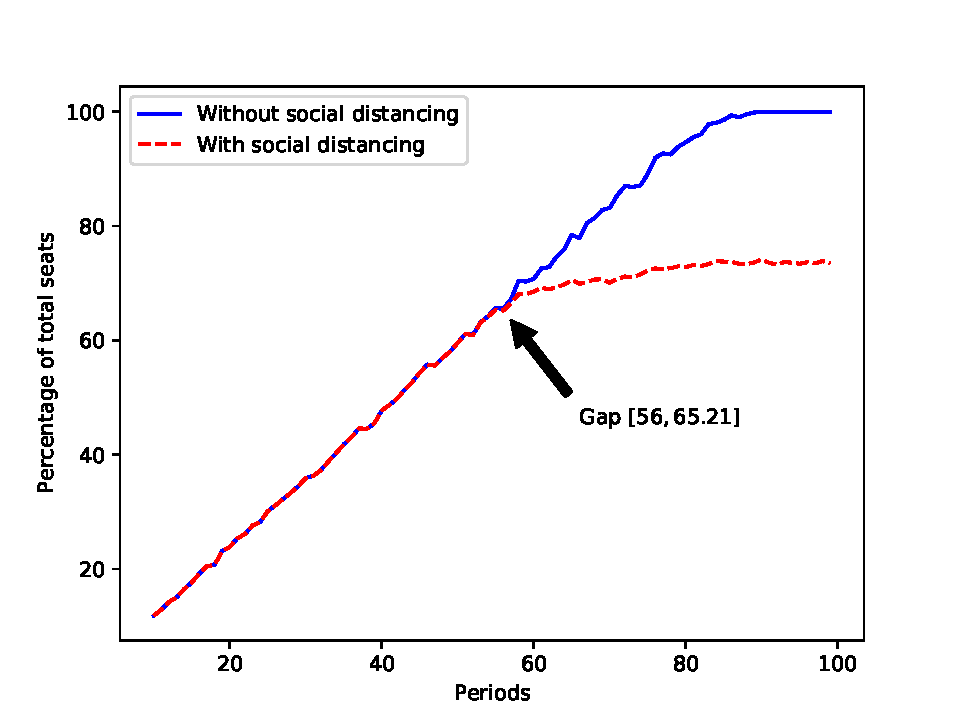
\includegraphics[width=0.48\textwidth]{./images/p1.pdf}}
            \subfigure[When $\gamma =1.9$]{
              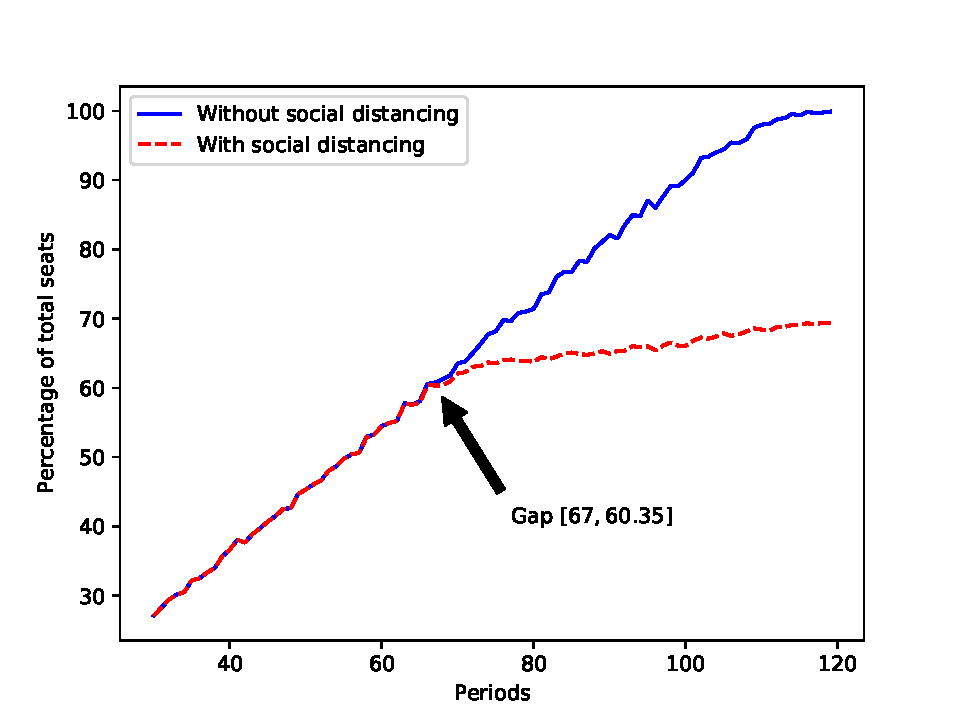
\includegraphics[width=0.48\textwidth]{./images/p2.pdf}}
          \end{figure}
        \scriptsize
        The gap point represents the first period where the number of people without social distancing is larger than that with social distancing and the gap percentage is the corresponding percentage of total seats.
    \end{frame}
      
    \begin{frame}{Estimation of Gap Point}
      \begin{figure}[ht]
        \centering
        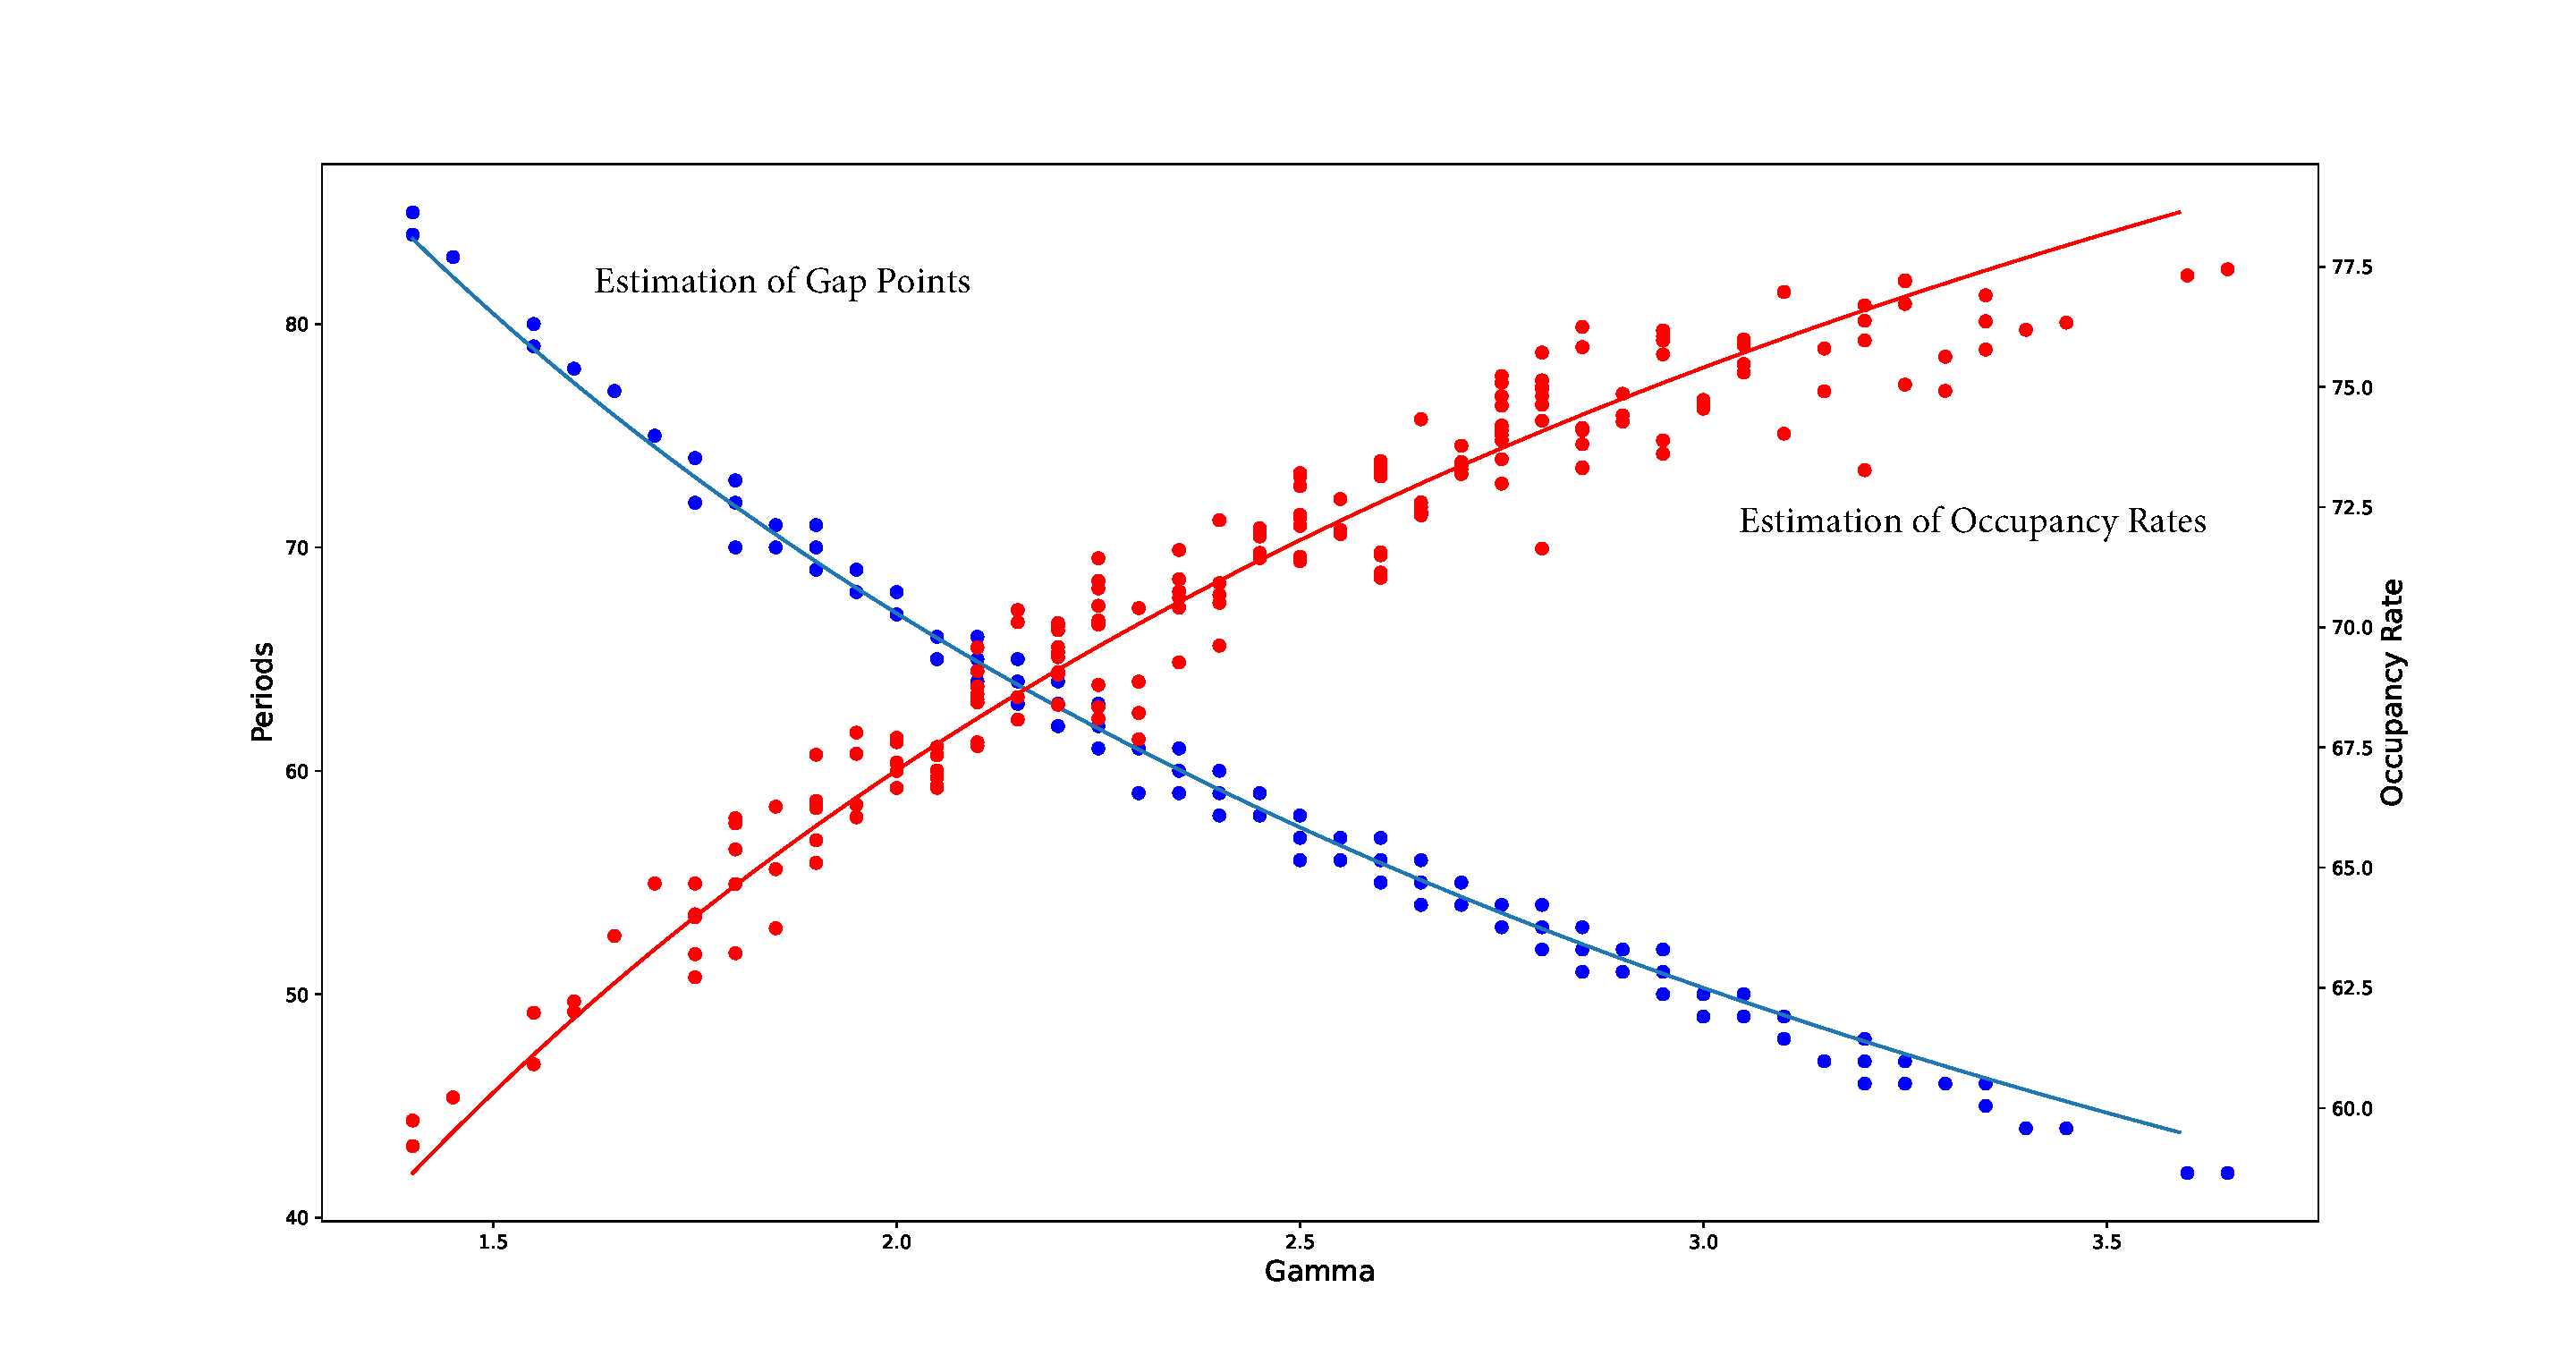
\includegraphics[width = 0.8\textwidth]{./images/gamma_estimation.pdf}
        \caption{Gap points with 200 probabilities}
    \end{figure}
    \scriptsize
    {\color{blue} Blue points}: period of the gap point.
    {\color{red} Red points}: occupancy rate of the gap point. 
    Gap points can be estimated.
    \end{frame}

    % We simulate 200 probabilities. For each probability, we run 100 instances to calculate the gap point and the corresponding occupancy rate. 
    
    % The point in the figure is the average of 100 instances. 
    % 


    \begin{frame}{Make A Later Allocation}
      This setting is particularly applicable to larger venues, such as stadiums, where an immediate decision is made when a group arrives, but the actual allocation of seats for that group is deferred to a later time.

      \vspace{0.5cm}

      The critical part is to make the decision, thus, we choose the following policies associated with relaxation forms.

      \vspace{0.5cm}

      Policies: 

      \begin{itemize}
        \item Dynamic programming based heuristic
        \item Bid-price control
      \end{itemize}
    \end{frame}

      \begin{frame}{Performances of Different Policies}
        \scriptsize
        \begin{table}[ht]
          \centering
          \begin{tabular}{|l|l|l|l|l|l|}
          \hline
           T & Probabilities &  DP1-L (\%) & Bid-L (\%) & DP1 (\%) & Bid (\%) \\
          \hline
          60  & [0.25, 0.25, 0.25, 0.25]  & 99.52 & 99.44 & 98.42 & 98.38 \\
          70  &   & 99.32 & 98.97 & 96.87 & 96.24 \\
          80  &   & 99.34 & 99.30 & 95.69 & 96.02 \\
          90  &   & 99.55 & 99.49 & 96.05 & 96.41  \\
          100 &   & 99.78 & 99.66 & 95.09 & 96.88 \\
          \hline
          60  & [0.25, 0.35, 0.05, 0.35]  & 99.50 & 99.37 & 98.26 & 98.25  \\
          70  &   & 99.40 & 98.97 & 96.62 & 96.06 \\
          80  &   & 99.46 & 99.24 & 96.01 & 95.89 \\
          90  &   & 99.59 & 99.35 & 96.77 & 96.62 \\
          100 &   & 99.77 & 99.61 & 97.04 & 97.14  \\
          \hline
          60  & [0.15, 0.25, 0.55, 0.05]  & 99.57 & 99.54 & 98.72 & 98.74 \\
          70  &   & 99.46 & 99.39  & 96.38 & 96.90 \\
          80  &   & 99.50 & 99.30  & 97.75 & 97.87 \\
          90  &   & 99.34 & 99.44  & 98.45 & 98.69 \\
          100 &   & 99.34 & 99.55  & 98.62 & 98.94 \\
          \hline
          \end{tabular}
        \end{table}

    \end{frame}

% !TEX root = sum1.tex
\section{Conclusion}
In conclusion, this paper addresses the problem of dynamic seat assignment with social distancing in the context of a pandemic. We propose a practical algorithm that balances seat utilization rates and the associated risk of infection to obtain a final seat planning that satisfies social distancing constraints when groups arrive. Our approach provides a comprehensive solution for optimizing seat assignments while ensuring the safety of customers. Our contributions include establishing a deterministic model to analyze the effects of social distancing when demand is known, using Benders decomposition methods to obtain the optimal solution for scenario-based stochastic programming, and developing a seat assignment policy for the dynamic situation. Our results demonstrate significant improvements over baseline strategies and provide guidance for developing attendance policies. Overall, our study highlights the importance of considering the operational significance behind social distancing and provides a new perspective for the government to adopt mechanisms for setting seat assignments to protect people in the post-pandemic era. Our study demonstrates the efficiency of obtaining the final seat planning using our proposed algorithm. The results indicate that our policy yields a seat planning that is very close to the optimal result. 

% Moreover, our analysis provides managerial guidance on how to set the occupancy rate and largest size of one group under the background of pandemic.


% \begin{table}[H]
%     \centering
%     \caption{xxxx}
%     \begin{tabular}{cccc}
%  \hline
%  a & aaaaaaaaa & aaaaaaaaaaaaaa & aaaaaaaaaaaaaaaaaaaa \\
%  \hline
%  a & \makebox[5ex][r]{123} & \makebox[6ex][r]{123456} & \makebox[6ex][r]{1}\\
%  a & \makebox[5ex][r]{12345} & \makebox[6ex][r]{123} & \makebox[6ex][r]{123} \\
%  a & \makebox[5ex][r]{1} & \makebox[6ex][r]{1234} & \makebox[6ex][r]{123456} \\
%  \hline
%  \end{tabular}
%  \end{table}

\bibliographystyle{plain}
\bibliography{refe}

% !TEX root = sum1.tex

\section{Policies for Dynamic Situations}\label{policies}

\subsubsection*{Bid-price Control}
Bid-price control is a classical approach discussed extensively in the literature on network revenue management. It involves setting bid prices for different group types, which determine the eligibility of groups to take the seats. Bid-prices refer to the opportunity costs of taking one seat. As usual, we estimate the bid price of a seat by the shadow price of the capacity constraint corresponding to some row. In this section, we will demonstrate the implementation of the bid-price control policy. 

The dual of LP relaxation of problem \eqref{deter_upper} is:

\begin{equation}\label{bid-price_dual}
  \begin{aligned}
  \min \quad & \sum_{i=1}^{M} d_i z_i + \sum_{j= 1}^{N} L_j \beta_{j} \\
  \text {s.t.} \quad & z_{i} + \beta_j n_i \geq (n_i-\delta), \quad i \in \mathcal{M}, j \in \mathcal{N} \\
  & z_{i} \geq 0, i \in \mathcal{M}, \beta_{j} \geq 0, j \in \mathcal{N}.
  \end{aligned}
\end{equation}

In \eqref{bid-price_dual}, $\beta_{j}$ can be interpreted as the bid-price for a seat in row $j$. A request is only accepted if the revenue it generates is above the sum of the bid prices of the seats it uses. Thus, if its revenue is more than its opportunity costs, i.e., $i -\beta_{j} n_i \geq 0$, we will accept the group type $i$. And choose $j^{*} = \arg \max_{j} \{i -\beta_{j} n_i\}$ as the row to allocate that group.


\begin{lem}\label{bid-price}
 The optimal solution to problem \eqref{bid-price_dual} is given by $z_1 ,\ldots, z_{\tilde{i}} =0$, $z_{i} = \frac{\delta(n_i-n_{\tilde{i}})}{n_{\tilde{i}}}$ for $i = \tilde{i}+1, \ldots, M$ and $\beta_j = \frac{n_{\tilde{i}} - \delta}{n_{\tilde{i}}}$ for all $j$.
\end{lem}

The bid-price decision can be expressed as $i - \beta_j n_i = i - \frac{n_{\tilde{i}} - \delta}{n_{\tilde{i}}} n_i = \frac{\delta (i - \tilde{i})}{n_{\tilde{i}}}$. When $i < \tilde{i}$, $i - \beta_j n_i < 0$. When $i \geq \tilde{i}$, $i - \beta_j n_i \geq 0$. This means that group type $i$ greater than or equal to $\tilde{i}$ will be accepted if the capacity allows. However, it should be noted that $\beta_j$ does not vary with $j$, which means the bid-price control cannot determine the specific row to assign the group to. In practice, groups are often assigned arbitrarily based on availability when the capacity allows, which can result in a large number of empty seats.

The bid-price control policy based on the static model is stated below.

\begin{algorithm}[H]
  \caption{Bid-price Control Algorithm}\label{algo_bid}
  \For{$t =1, \ldots, T$}{
    {Observe group type $i$\;}
    {Solve the LP relaxation of problem \eqref{deter_upper} with $d_i^{t} = (T-t) \cdot p_i$ and $\mathbf{L}^{t}$\;
    Obtain $\tilde{i}$ such that the aggregate optimal solution is $x e_{\tilde{i}} + \sum_{i=\tilde{i}+1} ^{M} d_{i} e_{i}$\;}
    \eIf{$i \geq \tilde{i}$ and $\max_j{L_j^{t}} \geq n_i$}
    {Accept the group and assign the group to row $k$ such that $L_{k}^{t} \geq n_{i}$\;}
    {Reject the group\;}}
\end{algorithm}


\subsubsection*{Booking Limit Control}
The booking limit control policy involves setting a maximum number of reservations that can be accepted for each group type. By controlling the booking limits, revenue managers can effectively manage demand and allocate inventory to maximize revenue.

In this policy, we replace the real demand by the expected one and solve the corresponding static problem using the expected demand. Then for every type of requests, we only allocate a fixed amount according to the static solution and reject all other exceeding requests. When we solve the linear relaxation of problem \eqref{deter_upper}, the aggregate optimal solution is the limits for each group type. Interestingly, the bid-price control policy is found to be equivalent to the booking limit control policy.

When we solve problem \eqref{deter_upper} directly, we can develop the booking limit control policy.

\begin{algorithm}[H]
  \caption{Booking Limit Control Algorithm}\label{algo_booking}
  \For{$t =1, \ldots, T$}{
    {Observe group type $i$\;}
    {Solve problem \eqref{deter_upper} with $d_i^{t} = (T-t) \cdot p_i$ and $\mathbf{L}^{t}$\;
    Obtain the optimal solution, $x_{ij}^{*}$ and the aggregate optimal solution, $\mathbf{X}$\;}
    \eIf{$X_i > 0$}
    {Accept the group and assign the group to row $k$ such that $x_{ik} > 0$\;}
    {Reject the group\;}}
\end{algorithm}


\subsubsection*{DP-based Heuristic}
To simplify the complexity of the original dynamic programming problem, we can consider a simplified version by relaxing all rows to a single row with the same total capacity, denoted as $\tilde{L} = \sum_{j=1}^{N} L_j$. With this simplification, we can make decisions for each group arrival based on the relaxed dynamic programming. By relaxing the rows to a single row, we aggregate the capacities of all individual rows into a single capacity value. This allows us to treat the seat assignment problem as a one-dimensional problem, reducing the computational complexity. Using the relaxed dynamic programming approach, we can determine the seat assignment decisions for each group arrival based on the simplified problem.

Let $u$ denote the decision, where $u^{t} = 1$ if we accept a request in period $t$, $u^{t} =0$ otherwise. Similar to the DP in section \ref{sec_dynamic_seat}, the DP with one row can be expressed as:

$$V^{t}(l) =  \max_{u^{t} \in \{0,1\}} \left\{ \sum_{i} p_i [V^{t+1}(l-n_i u^{t})+ i u^{t}] + p_0 V^{t+1}(l)\right\} $$
with the boundary conditions $V^{T+1}(l) =0, \forall l \geq 0$, $V^{t}(0) =0, \forall t$.

After accepting one group, assign it in some row arbitrarily when the capacity of the row allows.

\begin{algorithm}[H]
  \caption{DP-based Heuristic Algorithm}\label{algo_dp_heuris}
  Calculate $V^{t}(l)$, $\forall t =2, \ldots, T; \forall l = 1, \ldots, L$\;
  $l^{1} \gets L$\;
  \For{$t =1, \ldots, T$}{
    {Observe group type $i$\;}
    \eIf{$V^{t+1}(l^{t}) \leq V^{t+1}(l^{t}-n_i) + i$}
    {Accept the group and assign the group to an arbitrary row $k$ such that $L_{k}^{t} \geq n_i$\;  
    }
    {Reject the group\;}}
\end{algorithm}

\subsubsection*{First Come First Served (FCFS) Policy}
For dynamic seat assignment for each group arrival, the intuitive but trivial method will be on a first-come-first-served basis. Each accepted request will be assigned seats row by row. If the capacity of a row is insufficient to accommodate a request, we will allocate it to the next available row. If a subsequent request can fit exactly into the remaining capacity of a partially filled row, we will assign it to that row immediately. Then continue to process requests in this manner until all rows cannot accommodate any groups.

\begin{algorithm}[H]
  \caption{FCFS Policy Algorithm}\label{algo_fcfs}
  \For{$t =1, \ldots, T$}{
    {Observe group type $i$\;}
    \eIf{$\exists k$ such that $L_{k}^{t} \geq n_i$}
    {Accept the group and assign the group to row $k$\;}
    {Reject the group\;}}
\end{algorithm}

\subsubsection*{Tie-Breaking Rule}
These policies will encounter ties when the group can be assigned to two or more rows.
For the booking limit control, we assign the group according to the seat planning. The same tie-breaking rule used in the DSA approach can be applied for the booking limit control policy.
For the other policies besides the booking limit control, we adopt the following rule for assigning groups to rows. We prioritize assigning the group to rows that have at least $n_M$ seats available. If the number of remaining seats for all rows are less than $n_M$, we assign the group to an arbitrary row that has enough capacity to accommodate the group.

\newpage


% !TEX root = sum1.tex

\section{Policies for Dynamic Situations}\label{policies}

\subsubsection*{Bid-price Control}
Bid-price control is a classical approach discussed extensively in the literature on network revenue management. It involves setting bid prices for different group types, which determine the eligibility of groups to take the seats. Bid-prices refer to the opportunity costs of taking one seat. As usual, we estimate the bid price of a seat by the shadow price of the capacity constraint corresponding to some row. In this section, we will demonstrate the implementation of the bid-price control policy. 

The dual of LP relaxation of problem \eqref{deter_upper} is:

\begin{equation}\label{bid-price_dual}
  \begin{aligned}
  \min \quad & \sum_{i=1}^{M} d_i z_i + \sum_{j= 1}^{N} L_j \beta_{j} \\
  \text {s.t.} \quad & z_{i} + \beta_j n_i \geq (n_i-\delta), \quad i \in \mathcal{M}, j \in \mathcal{N} \\
  & z_{i} \geq 0, i \in \mathcal{M}, \beta_{j} \geq 0, j \in \mathcal{N}.
  \end{aligned}
\end{equation}

In \eqref{bid-price_dual}, $\beta_{j}$ can be interpreted as the bid-price for a seat in row $j$. A request is only accepted if the revenue it generates is above the sum of the bid prices of the seats it uses. Thus, if its revenue is more than its opportunity costs, i.e., $i -\beta_{j} n_i \geq 0$, we will accept the group type $i$. And choose $j^{*} = \arg \max_{j} \{i -\beta_{j} n_i\}$ as the row to allocate that group.

% The bid-price is a term used to describe the marginal value or opportunity cost of a seat.

% According to Lemma \ref{sol_relax_deter}, there exists $h$ such that the aggregate optimal solution to relaxation of problem \eqref{deter_upper} takes the form $x e_{h} + \sum_{i=h+1} ^{M} d_{i} e_{i}$, $x = (L- \sum_{i = h+1}^{M} {d_i n_i})/ n_h$.
\begin{lem}\label{bid-price}
 The optimal solution to problem \eqref{bid-price_dual} is given by $z_1 ,\ldots, z_{\tilde{i}} =0$, $z_{i} = \frac{\delta(n_i-n_{\tilde{i}})}{n_{\tilde{i}}}$ for $i = \tilde{i}+1, \ldots, M$ and $\beta_j = \frac{n_{\tilde{i}} - \delta}{n_{\tilde{i}}}$ for all $j$.
\end{lem}

The bid-price decision can be expressed as $i - \beta_j n_i = i - \frac{n_{\tilde{i}} - \delta}{n_{\tilde{i}}} n_i = \frac{\delta (i - \tilde{i})}{n_{\tilde{i}}}$. When $i < \tilde{i}$, $i - \beta_j n_i < 0$. When $i \geq \tilde{i}$, $i - \beta_j n_i \geq 0$. This means that group type $i$ greater than or equal to $\tilde{i}$ will be accepted if the capacity allows. However, it should be noted that $\beta_j$ does not vary with $j$, which means the bid-price control cannot determine the specific row to assign the group to. In practice, groups are often assigned arbitrarily based on availability when the capacity allows, which can result in a large number of empty seats.

The bid-price control policy based on the static model is stated below.

\begin{algorithm}[H]
  \caption{Bid-price Control Algorithm}\label{algo_bid}
  \For{$t =1, \ldots, T$}{
    {Observe group type $i$\;}
    {Solve the LP relaxation of problem \eqref{deter_upper} with $d_i^{t} = (T-t) \cdot p_i$ and $\mathbf{L}^{t}$\;
    Obtain $\tilde{i}$ such that the aggregate optimal solution is $x e_{\tilde{i}} + \sum_{i=\tilde{i}+1} ^{M} d_{i} e_{i}$\;}
    \eIf{$i \geq \tilde{i}$ and $\max_j{L_j} \geq n_i$}
    {Accept the group and assign the group to row $k$ such that $L_{k} \geq n_{i}$\;  
    $\mathbf{L}^{t+1} \gets \mathbf{L}^{t} - n_i \mathbf{e}_{k}$\;}
    {Reject the group\; $\mathbf{L}^{t+1} \gets \mathbf{L}^{t}$\;}}
\end{algorithm}


\subsubsection*{Booking Limit Control}

The booking limit control policy involves setting a maximum number of reservations that can be accepted for each group type. By controlling the booking limits, revenue managers can effectively manage demand and allocate inventory to maximize revenue.

In this policy, we replace the real demand by the expected one and solve the corresponding static problem using the expected demand. Then for every type of requests, we only allocate a fixed amount according to the static solution and reject all other exceeding requests. When we solve the linear relaxation of problem \eqref{deter_upper}, the aggregate optimal solution is the limits for each group type. Interestingly, the bid-price control policy is found to be equivalent to the booking limit control policy.

When we solve problem \eqref{deter_upper} directly, we can develop the booking limit control policy.

\begin{algorithm}[H]
  \caption{Booking limit Control Algorithm}\label{algo_booking}
  \For{$t =1, \ldots, T$}{
    {Observe group type $i$\;}
    {Solve problem \eqref{deter_upper} with $d_i^{t} = (T-t) \cdot p_i$ and $\mathbf{L}^{t}$\;
    Obtain the optimal solution, $x_{ij}^{*}$ and the aggregate optimal solution, $\mathbf{X}$\;}
    \eIf{$X_i > 0$}
    {Accept the group and assign the group to row $k$ such that $x_{ik} > 0$\;  
    $\mathbf{L}^{t+1} \gets \mathbf{L}^{t} - n_i \mathbf{e}_{k}$\;}
    {Reject the group\; $\mathbf{L}^{t+1} \gets \mathbf{L}^{t}$\;}}
\end{algorithm}


\subsubsection*{Dynamic Programming Base-heuristic}
To simplify the complexity of the original dynamic programming problem, we can consider a simplified version by relaxing all rows to a single row with the same total capacity, denoted as $\tilde{L} = \sum_{j=1}^{N} L_j$. With this simplification, we can make decisions for each group arrival based on the relaxed dynamic programming. By relaxing the rows to a single row, we aggregate the capacities of all individual rows into a single capacity value. This allows us to treat the seat assignment problem as a one-dimensional problem, reducing the computational complexity. Using the relaxed dynamic programming approach, we can determine the seat assignment decisions for each group arrival based on the simplified problem.


% Let $v_{r}^{*}$ and $v^{*}$ denote the optimal values of problem \eqref{relax_deter} and \eqref{deter_upper}, respectively. After relaxation, assume that each row has a capacity of $L$ seats, which can be filled. For each seperate row, the maximum number of empty seats in each row is $s$. Then, the total number of empty seats in $N$ rows is given by $Ns$. Therefore, the biggest difference between $v_{r}^{*}$ and $v^{*}$ is the number of people accommodated in the $Ns$ empty seats.
% The difference between them is zero only when the groups corresponding to the optimal solution of problem \eqref{relax_deter} can be accommodated in $N$ rows. The numerical results indicate that this is the case for most scenarios, which suggests that a DP-based approach can be used to solve the dynamic seat assignment problem after all groups have arrived.

Let $u$ denote the decision, where $u^{t} = 1$ if we accept a request in period $t$, $u^{t} =0$ otherwise. Similar to the DP in section \ref{sec_dynamic_seat}, the DP with one row can be expressed as:

$$V^{t}(l) =  \max_{u^{t} \in \{0,1\}} \left\{ \sum_{i} p_i [V^{t+1}(l-n_i u^{t})+ i u^{t}] + p_0 V^{t+1}(l)\right\} $$
with the boundary conditions $V^{T+1}(l) =0, \forall l \geq 0$, $V^{t}(0) =0, \forall t$.

After accepting one group, assign it in some row arbitrarily when the capacity of the row allows.

\begin{algorithm}[H]
  \caption{Dynamic Programming Base-heuristic Algorithm}\label{algo_dp_heuris}
  Calculate $V^{t}(l)$, $\forall t =2, \ldots, T; \forall l = 1, \ldots, L$\;
  $l^{1} \gets L$\;
  \For{$t =1, \ldots, T$}{
    {Observe group type $i$\;}
    \eIf{$V^{t+1}(l^{t}) \leq V^{t+1}(l^{t}-n_i) + i$}
    {Accept the group and assign the group to an arbitrary row $k$ such that $L_{k} \geq n_i$\;  
    $L_{k}^{t+1} \gets L_{k}^{t} - n_i$, $l^{t+1} \gets l^{t} - n_i$\;}
    {Reject the group\;
    $L_{k}^{t+1} \gets L_{k}^{t}$, $l^{t+1} \gets l^{t}$\;}}
\end{algorithm}

\subsubsection*{First Come First Served (FCFS) Policy}
For dynamic seat assignment for each group arrival, the intuitive but trivial method will be on a first-come-first-served basis. Each accepted request will be assigned seats row by row. If the capacity of a row is insufficient to accommodate a request, we will allocate it to the next available row. If a subsequent request can fit exactly into the remaining capacity of a partially filled row, we will assign it to that row immediately. Then continue to process requests in this manner until all rows cannot accommodate any groups.

\begin{algorithm}[H]
  \caption{FCFS Policy Algorithm}\label{algo_fcfs}
  \For{$t =1, \ldots, T$}{
    {Observe group type $i$\;}
    \eIf{$\exists k$ such that $L_{k} \geq n_i$}
    {Accept the group and assign the group to row $k$\;  
    $L_{k} \gets L_{k} - n_i$\;}
    {Reject the group\;}}
\end{algorithm}





\newpage


% % !TEX root = sum1.tex

\subsection{Obtain Minimum Number of Rows to Cover Demand}

To find the minimum number of rows to satisfy the demand, we can formulate this problem as a cutting stock problem form and use the column generation method to obtain an approximate solution.

Similar to the concept of pattern in the CSP, let the $k$-th placing pattern of a line of seats with length $S$ into some of the $m$ group types be denoted as a vector $(t^k_1,t^k_2,\ldots,t^k_m)$. Here, $t^k_i$ represents the number of times group type $i$ is placed in the $k$-th placing pattern. For a pattern $(t^k_1,t^k_2,\ldots,t^k_m)$ to be feasible, it must satisfy: $\sum_{i=1}^m t^k_i s_i \leq S$, where $s_i$ is the size of group type $i$. Denote by $K$ the current number of placing patterns.


This problem is to decide how to place a total number of group type $i$ at least $g_i$ times, from all the available placing patterns, so that the total number of rows of seats used is minimized.

Immediately we have the master problem:

\[\begin{split}\mbox{min}\quad & \sum_{k \in K}^K x_{k}\\
 \mbox{s.t.} \quad & \sum_{k \in K}^K t_i^k x_k \geq d_i  \quad  \mbox{ for } i=1,\ldots,m \\
  & x_k \geq 0, \mbox{integer}\quad \mbox{for}~ k \in K,\ldots,K.\\
\end{split}\]

If $K$ includes all possible patterns, we can obtain the optimal solution by solving the corresponding IP. But it is clear that the patterns will be numerous, considering all possible patterns will be time-consuming.

Thus, we need to consider the linear relaxation of the master problem, and the optimal dual variable vector $\lambda$. Using $\lambda$ as the value assigned to each group type $i$, the next problem is to find a feasible pattern $(y_1,y_2,\ldots,y_m)$ that maximizes the product of $\lambda$ and $y$.


Then the corresponding sub-problem is:
\[\begin{split}\mbox{max}\quad & \sum_{i=1}^m \lambda_i y_{i}\\
        \mbox{s.t.} \quad & \sum_{i=1}^m w_i y_i \leq S  \\
        & y_i \geq 0, \mbox{integer}\quad \mbox{for}~ i=1,\ldots,m.\\
\end{split}\]

This is a knapsack problem, its solution will be used as an additional pattern in the master problem.
We should continue to add new pattern until all reduced costs are nonnegative. Then we have an optimal solution to the original linear programming problem.

But note that column generation method cannot gaurantee an optimal solution. If we want to reach the optimal solution, we should tackle with the integer formulation.

\begin{equation}
\begin{aligned}
\min \sum_{k \in K}^{K} y_{k} & \\
\sum_{k=1}^{K} x_{i k} & \geq d_{i} \quad i=1, \ldots, n \\
\sum_{i=1}^{n} a_{i} x_{i k} & \leq S y_{k} \quad k=1, \ldots, K \\
y_{k} & \in\{0,1\} \quad k=1, \ldots, K \\
x_{i k} & \geq 0 \text { and integer } i=1, \ldots, n ; k=1, \ldots, K
\end{aligned}
\end{equation}

$y_k =1$ if line $k$ is used and 0 otherwise, $x_{ik}$ is the number of times group $i$ is placed in row $k$, and $K$ is the upper bound on the number of the rows needed.


\end{document}
